\documentclass[12pt]{book}
\usepackage[a4paper,bindingoffset=0.2in,%
            left=0.75in,right=0.75in,top=1in,bottom=1in,%
            footskip=.25in]{geometry}
\usepackage{fancyhdr}
\setlength{\headheight}{15.2pt}
\usepackage[utf8]{inputenc}
\pagestyle{fancy}

\renewcommand{\chaptermark}[1]{\markboth{\thechapter.\ #1}{}}
\renewcommand{\sectionmark}[1]{\markright{\thesection\ #1}}
\fancyhead[LE,RO]{\textbf{\thepage}}
\fancyhead[LO]{\textbf{\rightmark}}
\fancyhead[RE]{\textbf{\leftmark}}
\fancyfoot{}
\fancypagestyle{plain}
{
    \fancyhf{}
}


\usepackage{amsmath}
\usepackage{amssymb}
\usepackage{hyperref}
\usepackage{mathtools}
\usepackage{xcolor}
\usepackage{enumitem}
\usepackage{tikz}
\usepackage{float}
\usepackage{common}


\usepackage{english-theorems}
\setcounter{tocdepth}{1}

\begin{document}
\tableofcontents
\clearpage
\ifodd\value{page}\else
\thispagestyle{empty}
\fi
\part{Abstract Algebra}
\chapter{Preliminary}
\(R \subset A \times A\) is an equivalence relations if 
\begin{description}
    \item [Reflexive:] \(\forall a \in A, (a,a) \in R\).
    \item [Symmetric:] \((a,b) \in R \implies (b,a) \in R\).
    \item [Transitive:] \((a,b) \in R, (b,c) \in R \implies (a,c) \in R\).
\end{description}

A binary relations can be also denoted as \(aRb\) whenever \((a,b) \in R\).

If \(A\) is a set and if \(\sim\) is an equivalence relation on \(A\), then the equivalence class of \(a \in A\) is the set \(\set<x \in A>{x \sim a}\) denoted by \(\EqClass{a}\).

\begin{theorem}
    Equivalence classes partition the set into mutually disjoint subsets and conversely, mutually disjoint subsets give rise to equivalence classes.
\end{theorem}

If \(S\) and \(T\) are non-empty sets, then a mapping from \(S\) to \(T\) is a subset \(M \subset S \times T\) such that for every \(s \in S\) there is a unique \(t \in T\) that \((s,t) \in M\). \(\sigma:S \to T\) maybe denoted as \(t = s \sigma\) or \(t = \func{\sigma}{s}\).


\chapter{Group Theory}
\section{Introduction}
\begin{definition}
    A set \(S\) equipped with an associative binary operation is a \textbf{semigroup}.
\end{definition}
A semigroup can have multiple left or right identities. However, if it has both left identity, \(e\), and right identity, \(f\), then those two are equal since \(e = ef = f\). Two sided identity are unique. We have the same story with inverses.

\begin{definition}
    A non-empty set of elements \(G\) together with a binary operation \(\circ\) are said to be a \textbf{group} if 
    \begin{description}
        \item[Closure:] \(\forall a,b \in G, a \circ b \in G\).
        \item[Associative:] \(\forall a,b,c \in G, (a \circ b ) \circ c = a \circ (b \circ c)\).
        \item[Identity:] \(\exists e \in G\) such that \(\forall a\in G, a \circ e = e \circ a = a\).  
        \item[Inverse:] \(\forall a \in G \; \exists b \in G\) such that \(a \circ b = b \circ a = e\).  
    \end{description}
\end{definition}

\begin{example}
    The set of \(n_{\cardinalTH}\) roots of unity forms a group under multiplication.
\end{example}
\begin{example}
    The interval \(\clop{0}{1}\) forms a group under the following operation.
    \begin{equation*}
        x + y = \begin{cases}
            x + y & x + y < 1\\
            x + y - 1 & x + y \geq 1
        \end{cases}
    \end{equation*}
    This is called the \textbf{group of real numbers modulu 1}.
\end{example}

\begin{example}
    The set of all symmetries of a regular \(n\)-gon forms a group under composition. i.e. applying two symmetries results in a another symmetry. This is called \textbf{dihedral group of order }\(n\), denoted by \(D_n\). We can easily show that \(\abs{D_n} = 2n\). 
\end{example}

\begin{example}
    The permutations of a set form a group under composition, called the \textbf{symmetric group}, denoted by \(S_n\) for finite sets of size \(n\).
\end{example}

\begin{example}
    The \textbf{general linear group}, \(\func{\GL_n}{\bbF}\) is set of all non-singular \(n\times n\) matrices from field \(\bbF\).
\end{example}

\begin{example}
    The \textbf{Heisenberg group}
    \begin{equation*}
        \func{H}{\bbF} = \set< \begin{bmatrix}
            1 & a & b \\
            0 & 1 &c \\
            0 & 0 & 1
        \end{bmatrix}> {a,b,c \in \bbF}.
    \end{equation*}
\end{example}

\begin{example}
    The \textbf{Quaternion group}, \(Q_8 = \set{1,-i,i,-i,j,-j,k,-k}\) with \(i^2 = j^2 = k^2 = -1, ij = -ji = k, jk =-kj = i, ki = -ik =j\).
\end{example}

\begin{definition}
    A group \(G\) is said to be \textbf{abelian} or \textbf{commutative} if for any two element \(a\) and \(b\) commute. i.e. \(a \circ b = b \circ a\).
\end{definition}

\begin{definition}
    The number of elements in a group is called the \textbf{order} of the group and it is denoted by \(\abs{G}\).
\end{definition}

\begin{definition}
    Let \(\angleBracket{a} = \set<a^n>{n \in \Integers}\). If for some choice of \(a\), \(G = \angleBracket{a}\), then \(G\) is said to be a \textbf{cyclic group}. More generally, for a set \(W \subset G\), \(\angleBracket{W} = \bigcap{W \subset H \subset G} H\) where \(H\) is a subgroup of \(G\).
\end{definition}

\begin{lemma}
    Given \(a,b \in G\) the equation \(ax = b\) and \(ya = b\) have unique solutions for \(x,y \in G\).
\end{lemma}

\begin{prooflemma}
    Note that \(a^{-1}\) and \(b^{-1}\) are unique. Therefore, \(x = a^{-1}b\) and \(y = ba^{-1}\) are unique.
\end{prooflemma}
\ \\ 
{\Large{\textbf{Exercises}}}
\begin{enumerate}
    \item Let \(S\) be a finite semi-group. Prove that there exists \(e \in S\) such that \(e^2 = e\).
    \begin{proof}
        Pick \(a \in S\) and consider \(a_i = a^{2^i}\) for \(i \geq 1\). After some point, \(a_i\)s repeat, by the pigeon hole principle. Let that point be \(a_j\). Therefore, for some \(m \geq 1\).
        \begin{equation*}
            a_j = (a_j)^{2^m}
        \end{equation*}
        Let \(e = a_j^{2^m - 1}\), then
        \begin{equation*}
            e^2 = a_j^{2^{m+1} - 2} = a_j^{2^{m}} a_j^{2^m - 2} = a_j a_j^{2^m - 2} = e
        \end{equation*}
        we are done.
    \end{proof}
    \item Show that if a group \(G\) is abelian, then for \(a,b \in G\) and any integer \(n\), \((ab)^n = a^n b^n\).
    \begin{proof}
        Induct over positive \(n\). It is trivially true for \(n = 1\). Suppose it is true for \(n = k\), then 
        \begin{equation*}
            (ab)^{k+1} = (ab)^k ab = a^k b^k a b = a^{k} a b^k b = a^{k+1}b^{k+1}
        \end{equation*}
        For negative \(n\), note that 
        \begin{equation*}
            (ab)^{-1} = b^{-1} a^{-1} = a^{-1} b^{-1} \implies (ab)^{n} = ((ab)^{-1})^{-n} = (a^{-1} b^{-1})^{-n} = a^{n} b^{n}
        \end{equation*}
        hence it is true for all integers \(n\).
    \end{proof}
    \item If a group has an even order, then there exists \(a \neq e\) such that \(a^2 = e\).
    \begin{proof}
        Let \(A = \set<g>{g \neq g^{-1}}\) and \(B = \set<g>{g = g^{-1}}\). Note that, \(\abs{A}\) is even since  \(g  \in A \implies g^{-1} \in A\). Moreover, \(\abs{G} = \abs{A} + \abs{B}\), therefore \(\abs{B}\) must be even and since \(e \in B\), \(\abs{B} \geq 2\).
    \end{proof}
    \item For any \(n > 2\) construct a non-abelian group of order \(2n\).
    \begin{proof}
        Consider \(\phi, \psi\) where \(\psi^n = \phi^2 = e \) and \(\psi \phi = \phi \psi^{-1}\). Then
        \begin{equation*}
            G = \set{I, \phi ,\psi, \psi^2, \dots ,\psi^{n-1}, \phi \psi, \dots , \phi \psi^{n-1}}
        \end{equation*}
        is a group of order \(2n\). Because, by the product rules defined, any combination of \(\psi\) and \(\phi\) can be reduced to \(\phi^b \psi^k\) where \(b = 0,1\) and \(k = 0,1 , \dots, n-1\). It is cleary non-abelian as well.
    \end{proof}
    \item Find the order of \(\func{\GL_2}{\Integers_p}\) and \(\func{\SL_2}{\Integers_p}\) for a prime \(p\).
    \begin{proof}
        \begin{align*}
            \abs{\func{\GL_2}{\Integers_p}} &= (p+1) p (p-1)^2\\
            \abs{\func{\SL_2}{\Integers_p}} &= (p+1) p (p-1)
        \end{align*}
        which be can be calculate with some basic casing.
    \end{proof}
    \item Prove that finiteness of \(\func{\GL_n}{\bbF}\) is equivalent to finiteness of \(\bbF\).
\end{enumerate}

\section{Subgroup}
\begin{definition}
    A non-empty subset \(H\) of a group \(G\) is called a \textbf{subgroup} if under the product in \(G\), \(H\) itself forms a group. \(H\) is a subgroup of \(G\) is denoted by \(H \leq G\). If \(H\) is proper subgroup of, \(H < G\).
\end{definition}

\begin{lemma}\label{lm:subgroupConditions}
    \(H\) is a subgroup of \(G\) if and only if 
    \begin{enumerate}
        \item \(\forall a,b \in H, ab \in H\).
        \item \(\forall a \in H, a^{-1} \in H\).
    \end{enumerate}
\end{lemma}

\begin{prooflemma}
  If \(H\) is a subgroup, then the conditions hold. Suppose \(H\) is a subset of \(G\) that satisfies the conditions. Then, 
  \begin{enumerate}
      \item \(e \in H\) since \((a \in H \implies a^{-1} \in H) \implies e = a a^{-1} \in H\).
      \item Associativity is inherited from \(G\).
  \end{enumerate}
  invertibility and closure are given from the conditions. Therefore, \(H\) is a subgroup.
\end{prooflemma}

\begin{lemma}
    If \(H\) is a non-empty finite subset of a group \(G\) and \(H\) is closed under multiplication, then \(H\) is a subgroup of \(G\).
\end{lemma}

\begin{prooflemma}
    Since \(H\) is non-empty there exists a \(a \in H\). By closure, \(a^n\) for positive integer \(n\), are also in \(H\). We know that for some \(N\), \(a^N = e\) and therefore \(a^{-1} = a^{N - 1} \in H\). By \href{lm:subgroupConditions}, \(H\) is a subgroup.
\end{prooflemma}

\begin{definition}
    Let \(G\) be a group and \(H\) a subgroup of \(G\). For \(a,b \in G\) we say that \(a\) is congruent to \(b \mod{H}\), written as \(a \equiv b \mod{H}\) if \(ab^{-1} \in H\).
\end{definition}

\begin{lemma}
    The relation \(a \equiv b \mod{H}\) is an equivalence relation.
\end{lemma}

\begin{prooflemma}
    We show the equivalence axioms:
    \begin{enumerate}
        \item for any \(a\), \(a \equiv a \mod H\) becuase, \(aa^{-1} = e \in H\).
        \item for any \(a,b\), \(a \equiv b \mod H \implies b \equiv a \mod H\) since \(ab^{-1} \in H \) because of invertibility implies that \( (ab^{-1})^{-1} = ba^{-1} \in H\).
        \item for any \(a,b,c\), \(a \equiv b \mod H, b \equiv c \mod H \implies a \equiv c \mod H\) since \(ab^{-1}, bc^{-1} \in H \) because of closure implies that \( ab^{-1} bc^{-1} = bc^{-1} \in H\).
    \end{enumerate}
\end{prooflemma}

\begin{definition}
    If \(H\) is a subgroup of \(G\) and \(a \in G\), then \(Ha = \set<ha>{h \in H}\) is a \textbf{right coset} of \(H\) in \(G\). Similary, \(aH = \set<ah>{h \in H}\) is a \textbf{left coset} of \(H\) in \(G\).
\end{definition}

\begin{lemma}\label{lm:cosetsAreEquivalenceClasses}
    For all \(a \in G\), 
    \begin{equation*}
        Ha = \set<x \in G>{a \equiv x \mod{H}}
    \end{equation*}
\end{lemma}

\begin{prooflemma}
    Suppose \(x \in G\) and \(x \equiv a \mod{H}\). That is, \(xa^{-1} = h\) for some \(h \in H\). Then, \(x = ha\). Suppose \(h \in H\) and \(x = ha\). Then, \(xa^{-1} = h\) and hence \(x \equiv a \mod{H}\).
\end{prooflemma}

This implies, two right/left coset of \(H\) are either identical or disjoint.

\begin{lemma}\label{lm:cosetsHaveSameCardinality}
    There is a one-to-one correspondence between any two right/left cosets of \(H\).
\end{lemma}

\begin{prooflemma}
    Let \(R_1,R_2\) be two right cosets of \(H\) with \(a_1 \in R_1\) and \(a_2 \in R_2\). Note that, \(R_1 = Ha_1\) and \(R_2 = Ha_2\), therefore the map \(g \mapsto ga_1^{-1} a_2\) is a bijective map from \(R_1\) to \(R_2\).
\end{prooflemma}

\begin{theorem}[Lagrange's theorem]
    If \(G\) is a finite group and \(H\) is a subgroup of \(G\), then \(\abs{H} \mid \abs{G}\).
\end{theorem}

\begin{proof}
    By \href{lm:cosetsAreEquivalenceClasses} and \href{lm:cosetsHaveSameCardinality}, and from finiteness of \(G\), the order of \(G\) is equal to the number of right cosets multiplied by the cardinality of a right coset which is equal to the order of \(H\). Hence, \(\abs{H} \mid \abs{G}\)
\end{proof}

\begin{definition}
    If \(H\) is a subgroup of \(G\), the \textbf{index} of \(H\) in \(G\) is the number of distince right cosets of \(H\), denoted by \([G:H]\) or \(\func{i_G}{H}\).
\end{definition}

\begin{definition}
    Let \(G\) be a group and \(a \in G\), then the \textbf{order} or \textbf{period} of \(a\) is the least positive integer \(m\) such that \(a^m = e\). If no such integer exists we say that \(a\) is of infinite order. The order of \(a\) is denoted by \(\func{\ord_G}{a}\).
\end{definition}

\begin{corollary}
    If \(G\) is a finite group, then 
    \begin{enumerate}
        \item \(\abs{G} = \func{i_G}{H} \abs{H}\).
        \item \(\func{\ord_G}{a} \mid \abs{G}\).
        \item \(a^{\abs{G}} = e\).
        \item If \(\abs{G}\) is a prime, then \(G\) is cyclic.
    \end{enumerate}
\end{corollary}

Let \(A\) be a non-empty subset of \(G\). The smallest subgroup of \(G\) that contains \(A\) is denoted by \(\angleBracket{A}\) 
\begin{equation*}
    \angleBracket{A} = \bigcap_{\substack{A \subset H\\ H \leq G}} H
\end{equation*}

\begin{lemma}
    Let \(A\) be a non-empty subset of \(G\). Let 
    \begin{equation*}
        \bar{A} = \set<a_1^{\epsilon_1}a_2^{\epsilon_2}\dots a_n^{\epsilon_n}>{n \in \Integers^+_0, a_i \in A, \epsilon_i = \pm 1}
    \end{equation*}
    . Then \(\angleBracket{A} = \bar{A}\).
\end{lemma}

\begin{proof}
    First note that \(\bar{A}\) is a subgroup of \(G\) that contains \(A\), hence \(\angleBracket{A} \subset \bar{A}\). Moreover, since \(\angleBracket{A}\) is a subgroup of \(G\) that contains \(A\), then \(a_i^{\epsilon_i} \in \angleBracket{A}\), hence their product is in \(\angleBracket{A}\) as well. That is, \(\bar{A} \subset \angleBracket{A}\), thus \(\angleBracket{A} = \bar{A}\).
\end{proof}

\begin{definition}
    Let \(H,K \leq G\). The \textbf{join} of subgroups \(H\) and \(K\) denoted by \(\angleBracket{H,K}\) is the smallest subgroup which contains both subgroups.
\end{definition}

Subgroups of a groups can be represented by a lattice such as below.

\begin{figure}[H]
    \centering
    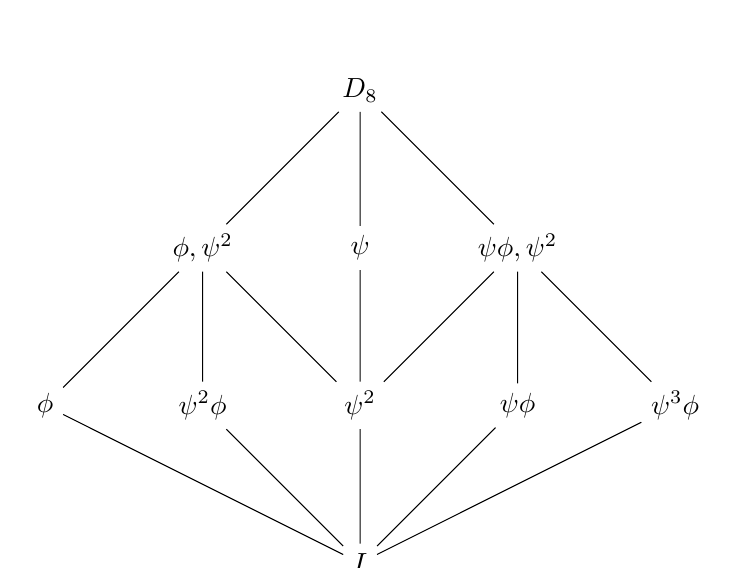
\begin{tikzpicture}[node distance=2cm]
    \node(D8) {$D_8$};
    \node(r)   [below of=D8] {$\angleBracket{\psi}$};
    \node(sr2) [left of= r] {$\angleBracket{\phi,\psi^2}$};
    \node(rsr2) [right of=r]{$\angleBracket{\psi \phi,\psi^2}$};
    \node(r2)[below of=r] {$\angleBracket{\psi^2}$};
    
    \node(r2s) [left of=r2]{$\angleBracket{\psi^2 \phi}$};
    \node(s) [left of=r2s] {$\angleBracket{\phi}$};

    \node(rs)[right of=r2] {$\angleBracket{\psi \phi}$};
    \node(r3s)[right of= rs] {$\angleBracket{\psi^3 \phi}$};
    \node(i)            [below of=r2]     {$\angleBracket{I}$};


    \draw (D8) -- (sr2)
    (D8) -- (r)
    (D8) -- (rsr2)
    (sr2) -- (s)
    (sr2) -- (r2s)
    (sr2) -- (r2)
    (r) -- (r2)
    (rsr2) -- (r2)
    (rsr2) -- (rs)
    (rsr2) -- (r3s)
    (s) -- (i)
    (r2s) -- (i)
    (r2) -- (i)
    (rs) -- (i)
    (r3s) -- (i);
\end{tikzpicture}

    \caption{The subgroup lattice of \(D_8\)}
\end{figure}
\ \\ 
{\Large{\textbf{Exercises}}}
\begin{enumerate}
    \item Suppose \(G\) is abelian group. Show that, the \textbf{torsion subgroup} \(\set<g \in G>{\func{\ord_G}{g} < \infty}\) is a subgroup of \(G\). Also, show that this is not generally true when \(G\) is non-abelian.
\end{enumerate}




\section{A counting principle}
Let \(H\) and \(K\) be two subgroups of \(G\), then 
\begin{equation*}
    HK = \set<hk>{h \in H, k \in K}
\end{equation*}

\begin{lemma}
    \(HK\) is a subgroup of \(G\) if and only if \(HK = KH\).
\end{lemma}
\begin{proof}
    Suppose \(HK\) is a subgroup. If \(hk \in HK\), then
    \begin{equation*}
        k^{-1}h^{-1} \in HK \implies k^{-1} \in H, h^{-1} \in K \implies k \in H,h \in K \implies hk  \in KH 
    \end{equation*}
    hence \(HK \subset KH\). If \(kh \in KH\), then 
    \begin{equation*}
        hk \in HK  \implies k^{-1} \in H, h^{-1} \in K \implies k \in H,h \in K \implies kh \in HK 
    \end{equation*}
    thus \(HK = KH\). Suppose \(HK = KH\) with \(h_1k_1, h_2k_2 \in HK\).
    \begin{enumerate}
        \item for closure we have 
        \begin{equation*}
            h_1k_1 h_2 k_2 = h_1 k_1(k_2' h_2') = h_1 (k_1k_2') h_2' = h_1 (k^{\ast} h_2') = h_1 h_2'' k^{\ast'}
        \end{equation*}
        \item for inverse 
        \begin{equation*}
            (h_1k_1)^{-1} = k_1^{-1} h_1^{-1} = h_1' k_1'
        \end{equation*}
    \end{enumerate}
\end{proof}
\begin{corollary}
    If \(H\) and \(K\) are subgroups of an abelian group \(G\), then \(HK\) is a subgroup of \(G\).
\end{corollary}

\begin{lemma}
    If \(H\) and \(K\) are finite subgroups \(G\), then 
    \begin{equation*}
        \abs{HK} = \dfrac{\abs{H} \abs{K}}{\abs{H \cap K}}
    \end{equation*}
\end{lemma}

\begin{prooflemma}
    If \(h_1 \in H \cap K\) then \(hk = (hh_1)(h_1^{-1}k)\). Therefore, \(hk\) appears at least \(\abs{H \cap K}\) times. If \(hk = h'k'\), then \(h'^{-1}h = k' k^{-1} \in H \cap K\). Let \(u = h'^{-1}h\) then \(h' = hu^{-1}\) and \(k' = uk\). Thus, all duplicates are accounted for.
\end{prooflemma}

\begin{corollary}
    If \(H\) and \(K\) are subgroups of \(G\) and \(\abs{H},\abs{K} > \sqrt{\abs{G}}\), then \(H \cap K \neq \set{e}\).
\end{corollary}

\begin{proof}
    \(HK \subset G\) therefore, \(\abs{HK} \leq \abs{G}\) and 
    \begin{equation*}
        \abs{G} \geq \abs{HK}  = \dfrac{\abs{H} \abs{K}}{\abs{H \cap K}} > \dfrac{\abs{G}}{\abs{H \cap K}} 
    \end{equation*}
    which implies that \(\abs{H \cap K} > 1\).
\end{proof}
\ \\ 
{\Large{\textbf{Exercises}}}
\begin{enumerate}
    \item Let \(G\) be a group such that the intersection of all of its subgroups that are different from \(\set{e}\) is different from \(\set{e}\). Prove that every element in \(G\) has finite order.
    \begin{proof}
        For the sake of contradiction, suppose \(a \in G\) has infinite order. Then, \(a^k\) are all different and 
        \begin{equation*}
            \bigcup_{k = 1}^{\infty} \angleBracket{a^k} = \set{e}
        \end{equation*}
        which is a contradiction.
    \end{proof}
    \item Show that there is one-to-one correspondence between the right and left cosets of a subgroup.
    \item Suppose \(H\) and \(K\) are finite index subgroups in \(G\). Show that \(H \cap K\) is a finite subgroup in \(G\).
    \begin{proof}
        Let \(Ha_1, \dots , Ha_n\) be the right cosets of \(H\) in \(G\) and \(Kb_1, \dots , Kb_m\) be the right costs of \(K\) in \(G\). Then, 
        \begin{equation*}
            G = G \cap G = \bigcap_i Ha_i \cap \bigcap_j Kb_j = \bigcap_{i,j} Ha_i \cap Kb_j
        \end{equation*}
        Suppose \(Ha_i \cap Kb_j\) is not empty. Let \(g \in Ha_i \cap Kb_j\), then \(Hg = Ha_i\) and \(Kg = Kb_j\). Thus, 
        \begin{equation*}
            Ha_i \cap Kb_j = Hg \cap Kg = (H \cap K)g
        \end{equation*}
        Therefore, \(Ha_i \cap Kb_j\) are either empty or a right coset of \(H \cap K\). Since there finitely many \(Ha_i \cap Kb_j\), there finitely many right cosets of \(H \cap K\) in \(G\). Moreover, \(\squareBracket{G:H \cap K} \leq \squareBracket{G:H} \squareBracket{G:K}\) by this construction. Note that, \(H \cap K\) is finite index in \(H\), and let \((H \cap K)c_1, \dots , (H \cap K)c_l\) be the right cosets of \(H \cap K\) in \(H\). We claim that \((H \cap K)c_ra_i\) are the right cosets of \(H \cap K\) in \(G\). By definition, for each \(x \in G\), there exists \(i\) such that \(x \in Ha_i\)and hence \(x = ha_i\) for some \(h \in H\). Similary, there exists \(r\) such that \(h \in (H \cap K)c_r\) and hence \(h = fc_r\) for some \(f \in H \cap K\). Therefore, \(x = fc_ra_i\) and \(x \in (H \cap K)c_ra_i\). Lastly, we must show that \((H \cap K)c_ra_i\) are disjoint. Consider \((H \cap K)  c_{r_1}a_{i_1}\) and \((H \cap K)c_{r_2}a_{i_2}\). Since \((H \cap K)c_{r_1}, (H \cap K)c_{r_2} \subset H\), then 
        \begin{align*}
            (H \cap K)c_{r_1}a_{i_1} = (H \cap K)  c_{r_2}a_{i_2} &\implies a_{i_1} = a_{i_2}, (H \cap K)  c_{r_1} = (H \cap K)  c_{r_2}\\
            &\implies a_{i_1} = a_{i_2}, c_{r_1} = c_{r_2}
        \end{align*}
        As a result, \(\squareBracket{G:H \cap K} = \squareBracket{G:H} \squareBracket{H:H\cap K}\).
        \end{proof}
    \item Let \(H\) be a finite index subgroup in \(G\). Show that there is only finitely many subgroups of form \(aHa^{-1}\) in \(G\).
    \begin{proof}
        Let \(a_1H, \dots, a_nH\) be left cosets of \(H\). Then, \(Ha_1^{-1}, \dots, Ha_n^{-1}\) are right cosets of \(H\). Suppose \(aH = a_iH\), then \(Ha^{-1} = Ha_i^{-1}\) and therefore, \(aHa^{-1} = a_{i} H a_{i}^{-1}\). Since there are finitely many \(a_i H a_i^{-1}\), then there are finitely many \(aHa^{-1}\).
    \end{proof}
    \item If an abelian group has subgroups of orders \(m\) and \(n\), respectively, then show it has a subgroup whose order is the least common multiple of \(m\) and \(n\).
    \item Let \(G\) be a finite (abelian) group in which the number of solutions in \(G\) of the equation \(x^n = e\) is at most \(n\) for every positive integer \(n\). Prove that \(G\) must be a cyclic group.
\end{enumerate}


\section{Normal subgroups}
\begin{definition}
    A subgroup \(N\) of \(G\) is \textbf{normal} if \(\forall g \in G,n \in N,\ gng^{-1} \in N\).
\end{definition}

\begin{lemma}\label{lm:normalEquivalency}
    \(N\) is normal if and only if \(gNg^{-1} = N\) for every \(g \in G\).
\end{lemma}

\begin{prooflemma}
    By definition, \(gNg^{-1} \subset N\). Let \(n \in N\), then \(g^{-1}ng = n'\) for some \(n' \in N\). Hence, \(n \in gNg^{-1}\) for all \(n \in N\).
\end{prooflemma}

\begin{lemma}
    \(N\) is a normal subgroup if and only if every left coset of \(N\) is a right coset.
\end{lemma}

\begin{prooflemma}
    If \(N\) is normal, then by \ref{lm:normalEquivalency}, \(gN = Ng\) for all \(g\). Suppose, for all \(g \in G\), \(gN = Nh\) for some \(h \in G\). Then, \(h = gn \implies gN = Ngn\) for \(n \in N\). This implies, \(gNn^{-1} = gN = Ng\) and therefore, \(gNg^{-1} = N\) which by \ref{lm:normalEquivalency} means that \(N\) is normal.
\end{prooflemma}

\begin{lemma}
    \(N\) is a normal subgroup if and only if the product of two right cosets of \(N\) is a right coset as well.
\end{lemma}

\begin{prooflemma}
    If \(N\) is normal, then 
    \begin{equation*}
        Na Nb = N (aN)b = N (Na)b = Nab
    \end{equation*}
    Then, suppose \(NaNb = Nc\) for all \(a,b \in G\) and some \(c \in G\). This implies \(NaNb = Nab\) and therefore, \(NaNa^{-1} = N \implies NaN = Na\).
    \begin{align*}
        NaN = Na &\implies \forall n, an \in Na \implies  aN \subset Na\\
        Na^{-1}N = Na^{-1} &\implies \forall n \exists n', a^{-1}n = n'a^{-1} \implies na = an' \implies Na \subset aN \\
    \end{align*}
    therefore, \(aN = Na\).
\end{prooflemma}

\begin{definition}
    \(G/N\) is called a \textbf{quotient group} is the set of all right cosets of \(N\).
\end{definition}

\begin{theorem}
    If \(N\) is normal in \(G\), then \(G/N\) is a group. Furthermore, for finite \(G\), \(\abs{G/N} = \frac{\abs{G}}{\abs{N}}\).
\end{theorem}

\begin{proof}
    Checking axioms is pretty easy. Note that, \(\abs{G/N} = \func{i_G}{N}\).
\end{proof}
\ \\ 
{\Large{\textbf{Exercises}}}
\begin{enumerate}
    \item The groups in which all subgroups are normal are called \textbf{Dedekind groups}. Non-abelian dedekind groups are called \textbf{Hamiltonian groups}. Show that quaternion group is a Hamiltonian group.
    \item Show that if \(K\) is a normal subgroup of \(N\) and \(N\) is a normal subgroup of \(G\), then \(K\) is not necessarily a subgroup of \(G\).
    % TODO: Dihedral group
\end{enumerate}

\section{Homomorphism}
\begin{definition}
    A mapping \(\phi\) from a group \(G\) to another group \(\bar{G}\) is a \textbf{homomorphism} if for all \(a,b \in G\)
    \begin{equation*}
        \func{\phi}{ab} = \func{\phi}{a} \func{\phi}{b}
    \end{equation*}
\end{definition}

\begin{lemma}
    Suppose \(G\) is a group, \(N\) a normal subgroup of \(G\), \(\phi: G \to G/N\) given by \(\func{\phi}{x} = Nx\) for all \(x \in G\). Then, \(\phi\) is a homomorphism.
\end{lemma}

\begin{prooflemma}
    Note that \(\func{\phi}{xy} = Nxy\) and \(\func{\phi}{x} \func{\phi}{y} = NxNy = Nxy\).
\end{prooflemma}

\begin{definition}
    If \(\phi\) is a homomorphism of \(G\) into \(\bar{G}\), the \textbf{kernel} of \(\phi\), \(K_{\phi}\) is defined as \(K_{\phi} = \set<x \in G>{\func{\phi}{x} = \bar{e}}\).
\end{definition}

\begin{lemma}
    If \(\phi: G \to \bar{G}\) is a homomorphism, then  
    \begin{enumerate}
        \item \(\func{\phi}{e} = \bar{e}\).
        \item \(\func{\phi}{x^{-1}} = \bracket{\func{\phi}{x}}^{-1}\).
    \end{enumerate}
\end{lemma}

\begin{prooflemma}
    \begin{equation*}
        \func{\phi}{xe} = \func{\phi}{x} = \func{\phi}{x}\func{\phi}{e} \implies \func{\phi}{e} = \bar{e}
    \end{equation*}
    and 
    \begin{equation*}
        \func{\phi}{x^{-1}} \func{\phi}{x} = \func{\phi}{x^{-1}x} = \bar{e} \implies \func{\phi}{x^{-1}} = \bracket{\func{\phi}{x}}^{-1}
    \end{equation*}
    \
\end{prooflemma}

\begin{lemma}
    If \(\phi\) is a homomorphism, then \(K_{\phi}\) is a normal subgroup of \(G\).
\end{lemma}

\begin{prooflemma}
    Pick an arbitray \(x \in G\) and \(y \in K_{\phi}\). Then, 
    \begin{equation*}
        \func{\phi}{x y x^{-1}} = \func{\phi}{x} \func{\phi}{y} \func{\phi}{x^{-1}} = \bar{e}
    \end{equation*}
    hence, \(xyx^{-1} \in K_{\phi}\).
\end{prooflemma}

\begin{lemma}\label{lm:homomorphismInverse}
    If \(\phi\) is a homomorphism, then the set all iverse images of \(\bar{g} \in \bar{G}\) under \(\phi\) is given by \(K_{\phi} x\) for any particular inverse image of \(\bar{g}\).
\end{lemma}

\begin{prooflemma}
    Suppose \(y\) is another inverse image of \(\bar{g}\). 
    \begin{align*}
        \func{\phi}{y} &= \bar{g} & \func{\phi}{x} &=\bar{g}\\
        \implies & \func{\phi}{yx^{-1}} = \bar{e} &\implies& yx^{-1} \in K_{\phi}
    \end{align*}
    which means \(y \in K_{\phi}{x}\). Also, clearly each \(y \in K_{\phi}{x}\) is an inverse image of \(\bar{g}\).
\end{prooflemma}

\begin{definition}
    A homomorphism \(\phi: G \to \bar{G}\) is an \textbf{isomorphism} if \(\phi\) is \underline{one-to-one}.
\end{definition}

\begin{definition}
    Two groups \(G\) and \(\bar{G}\) are \textbf{isomorphic} if there exists an isomorphism of \(G\) \underline{onto} \(\bar{G}\). Isomorphic groups are denoted by \(G \approx \bar{G}\).
\end{definition}

\begin{corollary}
    Let \(\phi\) be a homomorphism. Then, \(\phi\) is an isomorphism if and only if \(K_{\phi} = \set{e}\).
\end{corollary}

\begin{prooflemma}
    If \(\phi\) is an isomorphism, then it is injective and hence only \(e \in K_{\phi}\). Suppose \(K_{\phi} = \set{e}\), then we must show that \(\phi\) is a injective function. Suppose \(\func{\phi}{x} = \func{\phi}{y}\), then by \ref{lm:homomorphismInverse}, \(y x^{-1} \in K_{\phi}\). Thus, \(y = x\) and \(\phi\) is injective.
\end{prooflemma}

\begin{theorem}\label{thm:surjectiveHomomorphism}
    If \(\phi: G \to \bar{G}\) is a surjective homomorphism, then \(G/K_{\phi} \approx \bar{G}\)
\end{theorem}

\begin{prooflemma}
    Consider the following mapping, \(\psi: G/K_{\phi} \to \bar{G}\). For any \(X \in K/\phi\), \(\func{\psi}{X} = \func{\phi}{g}\) for some \(g \in X\). This is well-defined since if \(g,g' \in X\), then \(g' = xg\) for some \(x \in K_{\phi}\) and hence 
    \begin{equation*}
        \func{\phi}{g'} = \func{\phi}{g} \func{\phi}{x} = \func{\phi}{g}
    \end{equation*}
    Furthermore, \(\psi\) is injective. Suppose \(xK_{\phi},yK_{\phi} \in G/K_{\phi}\). Then,
    \begin{equation*}
        \func{\psi}{xK_{\phi}} = \func{\psi}{yK_{\phi}} \implies \func{\phi}{x} = \func{\phi}{y} \implies xy^{-1} \in K_{\phi}
    \end{equation*}
    which implies that \(x \in K_{\phi} y\) and hence \(K_{\phi} y = K_{\phi} x\). Moreover, this map is surjective. Let \(\bar{g} \in \bar{G}\). Since \(\phi\) is surjective, then there exists an inverse image \(g\). Therefore, \(\func{\psi}{gK_{\phi}} = \bar{g}\). Finally, we must show that \(\psi\) is a homomorphism. Since \(K_{\phi}\) is normal in \(G\) we have 
    \begin{equation*}
        \func{\psi}{xK_{\phi} y K_{\phi}} = \func{\psi}{xy K_{\phi}}= \func{\phi}{xy} = \func{\phi}{x}\func{\phi}{y} = \func{\psi}{xK_{\phi}} \func{\psi}{yK_{\phi}}
    \end{equation*}
    which concludes the proof.
\end{prooflemma}

Thus, we can find all homomorphic images of \(G\) by going through normal subgroups of \(G\).

\begin{definition}
    A group is \textbf{simple} if it has no non-trivial homomorphic images. i.e. it has no non-trivial normal subgroup.
\end{definition}

\begin{theorem}[Cauchy's theorem for finite abelian groups]\label{thm:CauchyForAbelian}
    Suoppose \(G\) is a finite abelian group, and \(p \mid \abs{G}\) where \(p\) is a prime number. Then, there is an element \(a \neq e\) such that \(a^p = e\).
\end{theorem}

\begin{proof}
    We induct over \(\abs{G}\). For \(G\) with a single element, the theorem is true trivially. If \(G\) has non-trivial subgroup \(H\), then \(G\) is cyclic and hence all its elements satisfy the condition. Suppose \(H\) is a non-trivial group of \(G\). Since \(G\) is abelian, then \(H\) is normal in \(G\). If \(p \mid \abs{H}\) then by induction we are done. Suppose otherwise, then \(p \mid \abs{G/H}\). Consder a set \(S\) where each element correspond to a right coset of \(H\). Clearly, there is a isomorphism between \(G/H\) and \(S\). Since \(S\) is a subgroup of \(G\) and \(p \mid \abs{S}\) by induction hypothesis we are done.
\end{proof}

\begin{theorem}[Sylow's theorem for finite abelian groups]
    Suppose the group \(G\) is a finite abelian group and \(p^{\alpha} \mid\mid \abs{G}\), then \(G\) has a unique subgroup of order \(p^{\alpha}\).
\end{theorem}

\begin{proof}
    We first prove the existence of such group. For \(\alpha = 0\), the claim holds trivially as \(\set{e}\) is a subgroup of order 1. . Suppose \(H = \set<x \in G>{x^{p^n} = e}\) is a subgroup of \(G\). Since \(p \mid \abs{G}\) there is a non identity element \(g\) such that \(g^p = e\). Hence \(g \in H\). We show that \(q \not \mid \abs{H}\) for any other prime \(q \neq p\). Since otherwise there is a an element \(h \in H\) where \(h \neq e \) and \(h^q = e\) by \ref{thm:CauchyForAbelian}. Since \(q\) and \(p^n\) are coprime, then \(h = e\) which is a contradiction. Lastly, we claim that \(p^{\alpha} \mid\mid \abs{H}\). Suppose the contrary that \(p^{\beta} \mid\mid \abs{H}\) for some \(\beta < \alpha\). Then, the quotient group of \(H\), \(p \mid \abs{G/H}\). By \ref{thm:CauchyForAbelian}, there is a right coset \(Hx \neq H\) such that \((Hx)^p = Hx^p = H\). This implies that \(x^p \in H\) which means \((x^p)^{p^n} = e\) for some \(n\). \(x^{p^{n+1}} = e \implies x \in H\). which is a contradtion. Thus, \(\abs{H} = p^{\alpha}\).

    Finally, suppose \(K \neq H\) is another subgroup of \(G\) such that \(\abs{K} = p^{\alpha}\). Then, note that 
    \begin{equation*}
        \abs{HK} = \dfrac{\abs{H} \abs{K}}{\abs{H \cap K}} = \dfrac{p^{2\alpha}}{\abs{H \cap K}} \implies p^{\gamma} \mid\mid \abs{HK}
    \end{equation*}
    However, this is a contradiction since  \(HK\) is a subgroup in \(G\). Therefore \(H\) is unique in \(G\).
\end{proof}

\begin{lemma}
    Suppose \(\phi: G \to \bar{G}\) is a surjective homomorphism and \(\bar{H}\) is a subgroup of \(\bar{G}\). Let \(H = \set<x \in G>{\func{\phi}{x} \in \bar{H}}\). Then, \(H\) is a subgroup of \(G\) and \(H \supset K_{\phi}\). If \(\bar{H}\) is normal in \(\bar{G}\), then \(H\) is normal. Moreover, this association sets up a one-to-one mapping from the set of all subgroups \(\bar{G}\) onto the set of all subgroups of \(G\) which contain \(K_{\phi}\).
\end{lemma}

\begin{prooflemma}
    Since \(\bar{e} \in \bar{H}\), then \(K_{\phi} \subset H\). Let \(x,y \in H\). \(xy \in H\) since \(\func{\phi}{xy} = \func{\phi}{x} \func{\phi}{y} \in \bar{H}\) and \(x^{-1} \in H\) since \(\func{\phi}{x^{-1}} = \bracket{\func{\phi}{x}}^{-1} \in \bar{H}\). Thus, \(H\) is a subgroup in \(G\). Assume that \(\bar{H}\) is normal and pick arbitray elements \(g \in G\) and \(h \in H\). 
    \begin{equation*}
        \func{\phi}{ghg^{-1}} = \func{\phi}{g} \func{\phi}{h} \bracket{\func{\phi}{g}}^{-1} \in \bar{H } \implies ghg^{-1} \in H
    \end{equation*}
    hence \(H\) is normal in \(G\). Let \(\bar{H},\bar{H'}\) be two subgroups of \(\bar{G}\) and \(H = \func{\phi^{-1}}{\bar{H}},H'= \func{\phi^{-1}}{\bar{H'}}\). Thus far we have proved that \(H,H' \supset K_{\phi}\) are subgroups of \(G\) and \(\phi^{-1}\) is surjective. If \(\bar{H} \neq \bar{H'}\), then there is an element \(x \in \bar{H}\) but \(x \notin \bar{H'}\). We should see that for any \(y = \func{\phi^{-1}}{x}\), \(y \subset H\) but \(y \notin H'\). Since \(\func{\phi}{y} = x \in \bar{H}\), then \(y \in H\). If \(y \in H'\), then \(\func{\phi}{y} = x \in \bar{H'}\) which is a contradiction. Therefore, \(\phi^{-1}\) is a injective as well. So \(\phi^{-1}\) is a bijection between the subgroups of \(\bar{G}\) and subgroups of \(G\) that contain \(K_{\phi}\).
\end{prooflemma}

\begin{theorem}
    Let \(\phi:G \to \bar{G}\) be a surjective homomorphism, \(\bar{N}\) a normal subgroup of \(\bar{G}\), and \(N = \set<x \in G>{\func{\phi}{x} \in N}\). Then, \(G/N \approx \bar{G}/\bar{N}\) and equivalently \(G/N \approx (G/K_{\phi})/(N/K_{\phi})\).
\end{theorem}

\begin{proof}
    The last equivalency results immediately from \ref{thm:surjectiveHomomorphism}. 
\end{proof}
\ \\ 
{\Large{\textbf{Exercises}}}
\begin{enumerate}
    \item Let \(U\) be a subset of a group \(G\). The subgroup generated by \(U\), denoted by \(\angleBracket{U}\) is the smallest subgroup that contains \(U\). Show that \(\angleBracket{U}\) exists and give a construction for it.
    \item Let \(U = \set<xyx^{-1}y^{-1}>{x,y \in G}\). In this case,\(\angleBracket{U}\) is usually written as \(\hat{G}\) and is called the \textbf{commutator subgroup} of \(G\).
    \begin{enumerate}
        \item Prove \(\hat{G}\) is normal in \(G\).
        \item Prove \(G/\hat{G}\) is abelian.
        \item If \(G/N\) is abelian, prove that \(N \supset \hat{G}\).
        \item Prove that if \(H\) is a subgroup of \(G\) and \(H \supset \hat{G}\), then \(H\) is normal in \(G\).
        \item Let \(G = \func{\GL_2}{\Reals}\) and \(N = \func{\SL_2}{\Reals}\). Show that \(N = \hat{G}\).
    \end{enumerate}
        \item Show that \(Q_8 \approx \func{\GL_2}{\Complex}\).
\end{enumerate}
\section{Cyclic groups}
We claim that cyclic groups of the same order are isomorphic. To show this, first consider the following proposition.

\begin{proposition}
    \begin{enumerate}
        \item If \(G = \angleBracket{g}\), then \(\abs{G} = \func{\ord_G}{g}\).
        \item If \(x \in G\) and \(x^m = x^n = e\), then \(x^{\func{\gcd}{m,n}} = e\).
    \end{enumerate}
\end{proposition}

\begin{theorem}
    Cyclic groups of the same order are isomorphic.
\end{theorem}

Given the above theorem, we let \(Z_n\) denotes the cyclic group of order \(n\), which is unique upto isomorphism.

\begin{proposition}
    Let \(G = \angleBracket{g}\).
    \begin{enumerate}
        \item If \(\func{\ord_G}{g} = \infty\), then \(G = \angleBracket{g^a}\) if and only if \(a = \pm 1\).
        \item If \(\func{\ord_G}{g} = n < \infty\), then \(G = \angleBracket{g^a}\) if and only if \(\func{\gcd}{n,a} = 1\). Hence, \(G\) has \(\func{\phi}{n}\) generators.
    \end{enumerate}
\end{proposition}

\begin{proposition}
    Let \(G = \angleBracket{g}\). All subgroups of \(G\) are cyclic. That is, if \(H \leq G\), then \(H = \angleBracket{g^d}\) for some \(d \in \Integers\).
    \begin{enumerate}
        \item If \(\func{\ord_G}{g} =  \infty\), then for all \(a,b \in \Integers^+_0\) with \(a\neq b\), \(\angleBracket{g^a} \neq \angleBracket{g^b}\). Moreover, for \(m \in \Integers\), \( \angleBracket{g^m} = \angleBracket{g^{\abs{m}}}\). This implies, that all  subgroups of \(G\) correspond bijectively with \(\Integers^+_0\).
        \item If \(\func{\ord_G}{g} = n < \infty\), then for all \(a \mid n\), \(\angleBracket{g^a}\) is a subgroup and for all \(m\),  \( \angleBracket{g^m} = \angleBracket{g^{\func{\gcd}{m,n}}}\). This implies, that all  subgroups of \(G\) correspond bijectively to divisors of \(n\).
    \end{enumerate}
\end{proposition}

\section{Automorphism}
\begin{definition}
    An isomorphism of a group onto iteslf is called an \textbf{automorphism}.
\end{definition}

\begin{lemma}
    If \(G\) is a group, then \(\func{\scrA}{G}\), the set of all automorphisms of \(G\) is also a group. The \(\func{\scrA}{G}\) is also denoted by \(\aut{G}\).
\end{lemma}

\begin{prooflemma}
    The \(\aut{G}\) is a group under composition. Suppose \(\theta,\phi, \psi \in \aut{G}\).
    \begin{enumerate}
        \item It is closed under composition. Since \(\phi, \theta\) are both bijective, then their composition is a bijection as well. Moreover, it is a homomorphisms
        \begin{equation*}
            \func{\phi}{\func{\psi}{xy}} = \func{\phi}{\func{\psi}{x} \func{\psi}{y}} = \func{\phi}{\func{\psi}{x}}\func{\phi}{\func{\psi}{y}}
        \end{equation*}
        therefore, \(\phi \circ \psi \in \aut{G}\).
        \item The identity is the identity transformation \(I\).
        \begin{equation*}
            I \circ \phi = \phi \circ I = \phi
        \end{equation*}
        \item the inverse of each automorphisms is its inverse map. Suppose \(\phi^{-1}\) is inverse of \(\phi\) 
        \begin{equation*}
            xy = \func{\phi}{\func{\phi^{-1}}{x}} \func{\phi}{ \func{\phi^{-1}}{y} } = \func{\phi}{\func{\phi^{-1}}{x} \func{\phi^{-1}}{x}} \implies \func{\phi^{-1}}{xy} = \func{\phi^{-1}}{x} \func{\phi^{-1}}{y} 
        \end{equation*}
        \item composition is associative 
        \begin{equation*}
            \phi \circ (\psi \circ \theta) = (\phi \circ \psi) \circ \theta
        \end{equation*}
    \end{enumerate} 
    for any maps \(\phi,\psi, \theta \) from \(G\) to \(G\).
\end{prooflemma}

\begin{example}
\(T_g:G \to G\) with \(xT_g = g^{-1}xg\). \(T_g\) is an automorphisms. \(T_g\) is called the \textbf{inner automorphism corresponding to \(g\)}. Let \(\func{\scrT}{G} = \set<T_g \in \aut{G}>{g \in G}\) is the \textbf{inner automorphism group} and is also denoted by \(\inn{G}\). \(\Psi: G \to \aut{G}\) given by \(g\Psi = T_g\) is a homomorphism. The kernel of \(\Psi\) is the \textbf{center} of \(G\), \(\func{Z}{G}\), the set of the elements that commute with all other elements. Note that, if \(g_o \in K_{\Psi}\), then \(T_{g_0} = I\), hence \(g_0^{-1}xg_0 = x\) implying \(g_0x = xg_0\) for all \(x \in G\). If \(g_0 \in \func{Z}{G}\), then \(xg_0 = g_0x\) for all \(x\), thus \(T_{g_0} = I\) and \(g_0 \in K_{\Psi}\).
\end{example}

\begin{lemma}
    \( G/Z\approx \inn{G}\).
\end{lemma}

\begin{prooflemma}
    Since \(K_{\psi} = Z\), this is an immediate result of \ref{thm:surjectiveHomomorphism}, by considering \(\Psi:G \to \inn{G}\).
\end{prooflemma}

\begin{lemma}
    Let \(G\) be a group and \(\phi\) be an automorphism of \(G\). If \(a \in G\) is of order \(\abs{a} > 0\), then \(\abs{\func{\phi}{a}} = \abs{a}\).
\end{lemma}

\begin{prooflemma}
    For any homomorphism \(\phi:G \to \bar{G}\), \(\abs{\func{\phi}{a}} \mid \abs{a}\) since 
    \begin{equation*}
        \func{\phi}{a}^{\abs{a}}= \func{\phi}{a^{\abs{a}}} = \func{\phi}{e} = \bar{e}
    \end{equation*}
    since both \(\phi\) and \(\phi^{-1}\) are homomorphism from \(G\) to \(G\), then 
    \begin{align*}
        &\abs{\func{\phi}{a}} \mid \abs{a}\\
        &\abs{\func{\phi^{-1}}{\func{\phi}{a}}} = \abs{a} \mid \abs{\func{\phi}{a}}\\
        \implies & \abs{\func{\phi}{a}} = \abs{a}
    \end{align*}
    \
\end{prooflemma}
\ \\ 
{\Large{\textbf{Exercises}}}
\begin{enumerate}
    \item A subgroup \(C\) of \(G\) is said to be a \textbf{characteristics subgroup} of \(G\) if \(CT \subset C\) for all automorphisms \(T\) of \(G\).    For any group \(G\), prove that the commutator subgroup \(\hat{G}\) is a characteristic subgroup of \(G\).
    \item Let \(G\) be a finite group, \(T\) an automorphism of \(G\) with property that \(xT=x\) if and only if \(x = e\). Suppose futher that \(T^2 = I\). Prove that \(G\) must be abelian.
    \item Let \(G\) be a finite group, \(T\) an automorphism of \(G\) that sends more than three-quarters of the elements of \(G\) onto their inverses. Prove that  \(xT = x^{-1}\) and that \(G\) is abelian.
    \item Let \(G\) be a group of order \(2n\). Suppose that half of the elements of \(G\) are of order \(2\), and the other half form a subgroup \(H\) of order \(n\). Prove that \(H\) is of odd order and is an abelian subgroup of \(G\).
\end{enumerate}
\section{Group Action}
\begin{definition}
    The \textbf{action} of a group \(G\) on a set \(A\) is a map \(\cdot: G \times A \to A\) which satisfies:
    \begin{enumerate}
        \item \(g \cdot (h \cdot a) = (gh) \cdot a\) for all \(g,h \in G\) and \(a \in A\).
        \item \(e \cdot a  = a\) for all \(a \in A\).
    \end{enumerate}
\end{definition}

Suppose \(\cdot\) is an action of \(G\) on \(A\). Then, \(\sigma_g : A \to A\) given by \(\func{\sigma_g}{a} = g \cdot a\) is a permutation of \(A\). Furthermore, \(\tau : G \to S_A\), \(g \mapsto \sigma_g\) is a homomorphism.

\begin{example}
    The \textbf{trivial action} is given by \(g \cdot a = a\) for all \(g \in G\) and \(a \in A\). In contrast, in a \textbf{faithful action} of \(G\) on \(A\), no \(g \neq e\) satisfies \(g \cdot a = a\) for all \(A\). In other words, in a faithful action, each element of \(G\) produces a different permutation. Thus \(\tau\) is an injective homomorphism.
\end{example}

Unless it is ambiguous, we omit the \(\cdot\), and write \(g \cdot a\) as \(ga\).

\begin{definition}
    The \textbf{kernel} of an action is \(\set<g \in G>{ga = a \; \forall a \in A}\).
\end{definition}

\begin{definition}
    The \textbf{stabilizer} of \(a\) is \(\set<g \in G>{ga = a}\).
\end{definition}
\section{Cayley's theorem}
\begin{theorem}[Cayley]
    Every group is isomorphic to a subgroup of \(\func{A}{S}\) for some set \(S\).
\end{theorem}

\begin{proof}
    Take \(S = G\) and let \(\tau_g: S \to S\) be given by \(\tau_g: x \mapsto xg\) for a \(g \in G\). We claim that \(\theta: G \to \func{A}{S}\) given by \(\theta: g \mapsto \tau_g\) is an isomorphism. First, we must show that \(\theta\) is well defined. That is, for all \(g \in G\), \(\tau_g \in \func{A}{S}\). Note that, if \(xg = yg\), then \(x = y\), hence \(\tau_g\) is injective. For every \(y \in G\), \(y = yg^{-1} \tau_g\), hence \(\tau_g\) is surjective. Thus, \(\tau_g \in \func{A}{S}\). Second, we show that \(\theta\) is a homomorphism. For all \(g,h,x \in G\), \(x(gh) = (xg)h\) therefore, \(\tau_{gh} = \tau_g \tau_h\). Finally, to show that \(\theta\) is an isomorphism, we must show that it is injective. If for all \(x \in G\), \(x\tau_g = x\tau_h\), then \(g = h\). Which was what was wanted.
\end{proof}

The construction above, describes a group \(G\) as a subgroup of \(\func{A}{G}\) that for finite \(G\), is of order \(\abs{G}!\). Too BIG. We wish to make it smaller. Consider the following results.

\begin{theorem}
    If \(G\) is a group, \(H\) a subgroup of \(G\), and \(S\) is the set of all right cosets of \(H\) in \(G\), then there is a homomorphism \(\theta: G \to \func{A}{S}\) and the kernel of \(\theta\) is the largest normal subgroup of \(G\) which is contained in \(H\).
\end{theorem}

\begin{proof}
    Let \(\tau_g: S \to S\) be given by \(Hx \tau_g = Hxg\) and then let \(\theta: G \to \func{A}{S}\) be given by \(\theta: g \mapsto \tau_g\). One can easily check that, \(\tau_g \in \func{A}{S}\) for all \(g\) and that \(\theta\) is a homomorphism. Suppose \(K\) is the kernel of \(\theta\). Since \(K\) is a kernel of a homomorphism, it is normal. Moreover, if \(g \in K\), then \(Hxg = Hx\) for all \(x \in G\). In particular, \(Hg = H\) which implies that \(g \in H\). As a result, \(K \subset H\). Lastly, suppose \(K'\) is another normal subgroup of \(G\) which is contained in \(H\). If \(g' \in K'\), then for all \(x \in G\), \(xg' x^{-1} \in K' \subset H'\). That is, there exists a \(h_x \in H\) such that \(xg' = hx\) which implies \(Hxg' = Hx\) for all \(x\). Therefore, \(g' \in K\) and \(K' \subset K\). Which was what was wanted.
\end{proof}

Given the above theorem, if \(H\) has no non-trivial normal subgroup of \(G\) inside it, then \(\theta\) is an isomorphism.

\begin{lemma}
    If \(G\) is a finite group, and \(H \neq G\) is a subgroup of \(G\) such that \(\abs{G} \nmid \func{i}{H}!\), then \(H\) must contain a non-trivial normal subgroup of \(G\). In particular, \(G\) is not simple.
\end{lemma}

\begin{proof}
    Suppose \(H\) contains no non-trivial normal subgroup of \(G\). Then, by preceding theorem, \(\theta \) is an isomorphism and \(G\) is isomorphic to a subgroup of \(\func{A}{S}\), where \(\func{A}{S} = \func{i}{H}!\). By Lagrange, theorem, \(\abs{G} \mid \func{i}{H}!\) which was what was wanted.
\end{proof}
\ \\ 
{\Large{\textbf{Exercises}}}
\begin{enumerate}
    \item Let \(\abs{G} = pq\), \(p > q\) are primes, prove 
    \begin{enumerate}
        \item \(G\) has a subgroup of order \(p\) and a subgroup of order \(q\).
        \item If \(q \nmid p - 1\), then \(G\) is cyclic.
        \item Given two primes, \(p\) and \(q\) with \(q \mid p - 1\), there exists a non-abelian group of order \(pq\).
        \item Any two non-abelian groups of order \(pq\) are isomorphic.
    \end{enumerate}
\end{enumerate}
\section{Permutation group}
Suppose \(S\) is a finite set having \(n\) elements \(x_1, \dots, x_n\). If \(\phi \in \func{A}{S}\), then \(\phi\) is a one-to-one correspondence and it can be represented as 
\begin{align*}
    \phi:& \begin{pmatrix*}
        x_1 & x_2 & \dots & x_n\\
        x_{i_1} & x_{i_2} & \dots & x_{i_n}
    \end{pmatrix*}
\intertext{ where \( x_{i_j} = \func{\phi}{x_j}\). More simply}
    & \begin{pmatrix*}
        1 & 2& \dots & n\\
        i_1 &i_2& \dots & i_n
    \end{pmatrix*} 
\end{align*}
By considering composition of \(\theta,\psi \in \func{A}{S}\), we can define multiplication on their representation. 

For \(\theta \in \func{A}{S}\) and \(a,b \in S\), \(a \overset{\theta}{\equiv} b \iff a = b \theta^i\) for some \(i \in \Integers\). This defines an equivalence relation. 

\begin{enumerate}
    \item \(a \overset{\theta}{\equiv} a \) for all \(a\), since \(a = a \theta^0\).
    \item \(a \overset{\theta}{\equiv} b\) implies \(b \overset{\theta}{\equiv} a\), since \(a = b \theta^{i} \implies b = a\theta^{-1}\).
    \item \(a \overset{\theta}{\equiv} b\) and \(b \overset{\theta}{\equiv} c\) implies \(a \overset{\theta}{\equiv} c\), since \(a = b \theta^i\) and \(b = c \theta^j\) implies \(a = c \theta^{i + j}\).
\end{enumerate}

We call the equivalence classes of \(s \in S\), the \textbf{orbit} of \(s\) under \(\theta\). The orbit of \(s\) consists of all elements in form of \(s \theta^i\), \(i \in \Integers\). If \(S\) is finite, then there is a smallest positive integer \(l = \func{l}{s}\) such that \(s\theta^l = s\). By \textbf{cycle} of \(\theta\) we mean the ordered set \((s,s\theta, \dots , s\theta^{l-1})\).

\begin{lemma}
    Every permutation is a product of its cycles.
\end{lemma}

\begin{prooflemma}
    Note that the cycles of a permutation are disjoint, and each is a permutation, hence their product is a permutation. Suppose \(\psi\) is the permutation of the product of cycles of \(\theta\). \(\psi\) is well-defined since the product of disjoint permutation is commutative. Futhermore, for each \(s \in S\), \(s\psi = \theta s\) thus, \(\theta = \psi\).
\end{prooflemma}

\begin{lemma}
    Every cycle can be written as a product of 2-cycle or \textbf{transpositions}.
\end{lemma}

\begin{prooflemma}
    Every \(m\)-cycle can be written as a product of 2-cycles. 
    \begin{equation*}
        \begin{pmatrix*}
            1 & 2& \dots & m
        \end{pmatrix*} = \begin{pmatrix*}
            1 & 2
        \end{pmatrix*}
        \begin{pmatrix*}
            2& 3
        \end{pmatrix*} \dots 
        \begin{pmatrix*}
            m-1& m
        \end{pmatrix*}
    \end{equation*}
\end{prooflemma}

\begin{definition}
    A permutation \(\theta \in S_n\) is said to be an \textbf{even permutation} if it can be represented as a product of an even number of transpositions, 
\end{definition}

The proof of well-definition of even permutation involves the polynomial \(\func{p}{x_1, \dots,x_n}\)
\begin{equation*}
    \func{p}{x_1,\dots, x_n} = \prod_{i < j} (x_i - x_j)
\end{equation*}
Define the action of \(\theta \in A(S_n)\) on the polynomial \(p\)
\begin{equation*}
    \theta \cdot p = \prod_{i < j} (x_{\func{\theta}{i}} - x_{\func{\theta}{j}})
\end{equation*}
It can be easily seen that \(\theta \cdot p = \pm p\). In fact, if \(\theta\) is a transposition, then \(\theta \cdot p = -p\). Since this is an action on \(p\), if \(\theta\) is the product of \(m\) transposition, \(\theta \cdot p = (-1)^m p\). Therefore, even permutations are well-defined. That is, no permutation can be written as a product of even number of transpositions and odd number of transpositions simultaneously.

Let \(A_n \subset S_n\) be the set of even permutations. \(A_n\) is a subgroup of \(S_n\) and it is called the \textbf{alternating group}. 
\begin{lemma}
    The alternating group is a normal subgroup of \(S_n\) of index \(2\), .
\end{lemma}
\begin{prooflemma}
    A way to prove this lemma, is to show that every odd permutation is in one coset of \(A_n\).
    
    Another way, is to show that \(\Psi:S_n \to W\) given by 
    \begin{equation*}
        \theta \Psi = \begin{cases}
            1 & \theta \text{ is even}\\
            -1 & \theta \text{ is odd}\\
        \end{cases}
    \end{equation*}
    is an onto homomorphism. \(W\) is the group of \(\set{1,-1}\) under multiplication. Then \(A_n\) is the kernel of \(\Psi\). Since \(S_n/A_n \approx W\), then 
    \begin{equation*}
        \dfrac{\abs{S_n}}{\abs{A_n}} = \abs{W} = 2
    \end{equation*}
    Which was what was wanted.
\end{prooflemma}
\ \\ 
{\Large{\textbf{Exercises}}}
\begin{enumerate}
    \item  
    \begin{enumerate}
        \item What is the order of an \(n\)-cycle.
        \item What is the order of the product of disjoint cycles of length \(m_1,m_2, \dots , m_k\).
        \item How do you find the order of a given permutation?
    \end{enumerate}
    \item Prove that \(A_5\) has no non-trivial normal subgroups.
    \item If \(n \geq 5\) prove that \(A_n\) is the only non-trivial normal subgroup in \(S_n\).
\end{enumerate}
\section{Another counting principle} 
\begin{definition}
    If \(a,b \in G\), then \(b\) is said to be a \textbf{conjugate} of \(a\) in \(G\), denoted by \(a \sim b\), if there exists an element \(c \in G\) such that \(b = c^{-1}ac\)
\end{definition}

\begin{lemma}
    Conjugacy is an equivalence relation on \(G\).
\end{lemma}

\begin{prooflemma}
    \begin{enumerate}
        \item \(a \sim a\) for all \(a \in G\), \(a = e^{-1}ae\).
        \item \(a \sim b \implies b \sim a\) for all \(a,b \in G\), since \(a = c^{-1}bc \) implies that \(b = cac^{-1}\).
        \item \(a \sim b, b \sim c \implies a \sim c\) for all \(a,b,c \in G\), since \(a = d^{-1}b d = d^{-1}e^{-1}ced = (ed)^{-1}c(ed)\).
    \end{enumerate}
\end{prooflemma}

For \(a\in G\) let \(\func{C}{a} = \set<x \in G>{x \sim a}\). \(\func{C}{a}\) is called the \textbf{conjugate class} of \(a \) in \(G\). It consists all elements in form of \(y^{-1}ay\) for \(y \in G\). Suppose \(G\) is a finite group and \(A\) is a set of representative of conjugacy classes. Then, 
\begin{equation*}
    \abs{G} = \sum_{a \in A} \abs{\func{C}{a}}
\end{equation*}

\begin{definition}
    Suppose \(a \in G\). The \textbf{normalizer} of \(a\) in \(G\), denoted by \(\func{N}{a}\), is the set of all elements that commute with \(a\), \(\func{N}{a} = \set<x \in G>{ax = xa}\).
\end{definition}

\begin{lemma}
    \(\func{N}{a}\) is a subgroup of \(G\).
\end{lemma}

\begin{prooflemma}
    Suppose \(x,y \in \func{N}{a}\), then \(a(xy) = (ax)y = (xa)y = x(ay) = x(ya) = (xy)a\). And \(x^{-1}a = ax^{-1}\) holds. Therefore, \(\func{N}{a}\) is a subgroup of \(G\).
\end{prooflemma}

\begin{theorem}\label{thm:SizeofConjugacyClass}
    If \(G\) is a finite group, then \(\abs{\func{C}{a}} = \func{i_G}{\func{N}{a}}\). i.e. the number of elements conjugate to \(a\) in \(G\) is the index of normalized of \(a\) in \(G\).
\end{theorem}

\begin{proof}
    Let \(S\) be the set of right cosets of \(\func{N}{a}\) in \(G\). Consider \(\varphi : S \to \func{C}{a}\) given by \(\varphi: \func{N}{a}g \mapsto g^{-1}ag\). This, function is well-defined since if \(\func{N}{a}g = \func{N}{a}h\), then \(g = nh\) for some \(n \in \func{N}{a}\). Then, \(g^{-1}ag = h^{-1}n^{-1}anh = h^{-1}ah\). Similary, it is injective. If \(\func{N}{a}g \varphi = \func{N}{a}h \varphi\), then \(g^{-1}ag = h^{-1}a h \implies a=(gh^{-1})a (hg^{-1}) \implies hg^{-1} \in \func{N}{a}\) hence \(\func{N}{a}g = \func{N}{a}h\). \(\varphi\) is clearly surjective. Suppose \(x \in \func{C}{a}\), then there exists \(g \in G\) such that \(x = g^{-1}ag\). Then, \(\func{N}{a}g \varphi = g^{-1}ag = x\). Therefore, \(\varphi\) is a bijection and \(\abs{\func{C}{a}} = \func{i_G}{\func{N}{a}}\).
\end{proof}
\begin{corollary}\label{cor:classEquation}
    The \textit{class equation} of \(G\)
    \begin{equation*}
        \abs{G} = \sum_{a \in A} \dfrac{\abs{G}}{\abs{\func{N}{a}}}
    \end{equation*}
\end{corollary}

Recall that the center \(\func{Z}{G}\) of a group \(G\) is the set of all \(a \in G\) such that \(ax = xa\) for all \(x \in G\). 

\begin{lemma}
    \(a \in \func{Z}{G}\) if and only if \(\func{N}{a} = G\). If \(G\) is finite, \(a \in \func{Z}{G}\) if and only if \(\abs{\func{N}{a}} = \abs{G}\).
\end{lemma}

\begin{prooflemma}
    It can be readily proven by applying the definitions.
\end{prooflemma}

\subsection{Applications of \ref{thm:SizeofConjugacyClass}}

\begin{theorem}
    If \(\abs{G} = p^n\) where \(p\) is a prime number, then \(\func{Z}{G} \neq \set{e}\).
\end{theorem}

\begin{proof}
    Let \(z = \abs{\func{Z}{G}}\). For each \(a \in \func{Z}{G}\), \(\abs{\func{C}{a} }= 1\). For each \(b \notin \func{Z}{G}\), \(\func{N}{a} \neq G\), hence \(\abs{\func{N}{a}} = p^{k}\) for some \(0 < k < n\). Therefore, \(\abs{\func{C}{a}} = p^{n - k}\) with \(n - k \geq 1\). Hence, 
    \begin{align*}
        p^n &= \sum_{a \in A} \abs{\func{C}{a}} \\
        &= \sum_{A \cap \func{Z}{G}} \abs{\func{C}{a}} + \sum_{A \cap (\func{Z}{G})^c} \abs{\func{C}{a}}\\
        &= z + \sum_{A \cap (\func{Z}{G})^c} \abs{\func{C}{a}}
    \end{align*}
    We have shown that, for \(a \notin \func{Z}{G}\), then \(p \mid \abs{\func{C}{a}}\), thus \(p \mid z\). Since \(e \in \func{Z}{G}\), then \(\func{Z}{G}\) contains at least \(p\) elements.
\end{proof}

\begin{corollary}
    If \(\abs{G} = p^2\) where \(p\) is a prime number, then \(G\) is abelian.
\end{corollary}

\begin{proof}
    Based on the proof last theorem, \(\abs{\func{Z}{G}}= p,p^2\). Suppose \(\abs{\func{Z}{G}} = p\) and \(a \notin \func{Z}{G}\). Then, \(\func{Z}{G} \subsetneq \func{N}{a}\). By Lagrange's theorem, \(\abs{\func{N}{a}} \mid \abs{G}\), thus \(\abs{\func{N}{a}} = p^2\) which means \(a \in \func{Z}{G}\), a contradiction. Therefore, \(\abs{\func{Z}{G}} = p^2\) and \(G\) is abelian.
\end{proof}

\begin{theorem}[Cauchy]
    If \(p\) is a prime number and \(p \mid \abs{G}\), then \(G\) has an element of order \(p\).
\end{theorem}

\begin{proof}
    If \(\abs{G} = p\), then \(G\) is cyclic and the theorem holds. Suppose, the statement is true for all groups with \(\abs{G} = pk\) for \(1 \leq k \leq n-1\), we will show that it is also true for \(\abs{G} = np\). That is, we will prove the theorem by induction. If \(G\) has a non-trivial subset \(H\) where \(p \mid \abs{H}\), then we would be done. Suppose, that \(p\) divides the order of no non-trivial subgroup of \(H\). Consider the normalizer subgroups, \(\func{N}{a}\). If a normalizer subgroup is trivial, then \(\func{N}{a} = G\) and hence \(a \in \func{Z}{G}\). If it is not trivial, then its index divides \(p\). 
    \begin{equation*}
        p^n = z + \sum_{A \cap (\func{Z}{G})^c} \abs{\func{C}{a}} \implies p \mid z
    \end{equation*} 
    That is \(p \mid \abs{\func{Z}{G}}\). Therefore, \(\func{Z}{G} = G\) which means \(G\) is abelian. By Cauchy's theorem for abelian groups, there exists \(a \neq e\) such that \(a^p = e\).
\end{proof}

Recall that every permutation in \(S_n\) can be decomposed into disjoint cycles. We shall say a permutation \(\sigma \in S_n\) has the \textbf{cycle decomposition} \(\set{n_1, \dots , n_r}\) if it can be written as product of disjoint cycles of length \(n_1, \dots ,n _r\) with \(n_1 \leq n_2 \leq \dots \leq n_r\).

\begin{lemma}
    Two permutations in \(S_n\) are conjugate if and only if they have the same cycle decomposition.
\end{lemma}

\begin{prooflemma}
    Conjugation in \(S_n\) leaves the cyclic decomposition unchanged. Also, for any two permutations with the same cyclic decomposition, we can find a \(\theta \in S_n\) such that \(\sigma_1 = \theta^{-1} \sigma_2 \theta\).
\end{prooflemma}
\begin{corollary}
    The number of conjugate classes in \(S_n\) is \(\func{p}{n}\), the number of partitions of \(n\).
\end{corollary}
\begin{prooflemma}
    Every conjugate class corresponds to a partition of \(n\).
\end{prooflemma}

\ \\ 
{\Large{\textbf{Exercises}}}
\begin{enumerate}
    \item 
\end{enumerate}
\section{Centralizers and Normalizers}
\begin{definition}
    Let \(A\) be a non-empty subset of \(G\). \(\func{C_G}{A} = \set<g \in G>{gag^{-1} = a \; \forall a \in A}\) is called the \textbf{centralizer} of \(A\) in \(G\). \(\func{N_G}{A} = \set<g \in G>{gAg^{-1} = A}\) is the \textbf{normalizer} of \(A\) in \(G\). 
\end{definition}
\begin{example}
    \(\func{Z}{G} = \func{C_G}{G}\). 
\end{example}

\begin{proposition}
    For all \(A \subset G\), \(\func{C_G}{A}\) and \(\func{N_G}{A}\) are subgroups of \(G\) and 
    \begin{equation*}
        \func{C_G}{A} \leq \func{N_G}{A} \leq G
    \end{equation*}
\end{proposition}

\begin{proposition}
    \(\func{C_G}{\func{Z}{G}} = G\).
\end{proposition}

\begin{proposition}
    If \(A \subset B\), then \(\func{C_G}{B} \leq \func{C_G}{A}\).
\end{proposition}
\begin{proposition}
    If \(H \leq G\), then \(H \leq \func{N_G}{H}\) and \(H \leq \func{C_G}{H}\) if and only if \(H\) is abelian. Furthermore, \(\func{N_H}{A} =\func{N_G}{A} \cap H\) and \(\func{N_H}{A} \leq H\).
\end{proposition}

\begin{proposition}
    If \(A \subset G\), then \(\func{N_G}{A} \geq \func{Z}{G}\).
\end{proposition}

\begin{proposition}
    \(\func{Z}{\func{H}{\bbF}} \approx \bbF\), the additive group of the field \(\bbF\).
\end{proposition}

\section{Sylow's theorem}



\begin{theorem}[Sylow]
    If \(p\) is a prime number and \(p^{\alpha} \mid \abs{G}\), then \(G\) has a subgroup of order \(p^{\alpha}\).
\end{theorem}
We give three proofs for this theorem.
\begin{proof}
    Let \(\abs{G} = p^{\alpha}m\) where \(p^r \mid\mid m\) for some \(r \geq 0\). Consider \(\calM\), the set of all \(p^{\alpha}\)-element subsets of \(G\). Clearly, \(\abs{\calM} = \binom{p^{\alpha} m}{p^{\alpha}}\). Let \(\func{e_p}{n}\) be \(p^{\func{e_p}{n}} \mid\mid n\).
     We claim that \(p^r \mid \mid \abs{\calM}\). Note that 
    \begin{equation*}
        \func{e_p}{\abs{\calM}} =  \func{e_p}{(p^{\alpha}m)!} -  \func{e_p}{(p^{\alpha})!} -  \func{e_p}{(p^{\alpha}(m - 1))!}
    \end{equation*}
    For any \(m\) and \(\alpha\)
    \begin{equation*}
        \func{e_p}{(p^{\alpha}m)!} = m \func{e_p}{(p^{\alpha})!} + \func{e_p}{m!}
    \end{equation*}
    therefore,
    \begin{align*}
        \func{e_p}{\abs{\calM}} &=  \func{e_p}{(p^{\alpha}m)!} -  \func{e_p}{(p^{\alpha})!} -  \func{e_p}{(p^{\alpha}(m - 1))!}\\
        &= \func{e_p}{m!} - \func{e_p}{(m-1)!} \\
        &= \func{e_p}{\dfrac{m!}{(m-1)!}} \\
        &= \func{e_p}{m}
    \end{align*}
    which proves the claim. Define the equivalence relation \(\sim\) on \(\calM\) as following. \(M_1, M_2 \in \calM\) are equivalent if there exists a \(g \in G\) such that  \(M_1 = M_2 g\). There is at least one equivalence class that the number of elements in that class does not divide \(p^{r+1}\). As otherwise, \(p^{r+1}\mid \abs{\calM}\) which is a contradiction. Suppose \(\set{M_1, \dots, M_n}\) where \(p^{r+1} \nmid n\) is that equivalence class. Let \(H = \set<g \in G>{M_1 g = M_1}\). It can be easily shown that \(H\) is a subgroup of \(G\). We will show that \(\func{i_G}{H} = n\). Let \(\phi: Hg \mapsto M_1 g\)
    \begin{itemize}
        \item \(\phi\) is well-defined. Let \(Hg_1 = Hg_2\), then \(g_2 = hg_1\) where \(h \in H\). Hence 
        \begin{equation*}
            M_1 g_2 = M_1 hg_1 = M_1 g_1
        \end{equation*}
        \item \(\phi\) is injective. Suppose \(M_1 g_1 = M_1 g_2\), then \(M_1 g_1g^{-1}_2 = M_2\) thus \(g_1g_2^{-1} \in H \implies H g_1 = H g_2\).
        \item \(\phi\) is clearly surjective. 
    \end{itemize}
    Note that \(\set<M_1g>{g \in G} = \set{M_1, \dots, M_n}\) by definition. Then, \(\func{i_G}{H} = n\). which implies \(p^{\alpha} \mid \abs{H}\). For each \(m_1 \in M_1\), \(m_1 H_1 \subset M_1\), therefore, \(H\) has at most \(p^{\alpha}\) distinct elements. Thus \(\abs{H} = p^{\alpha}\).
\end{proof}

\begin{corollary}
    If \(p^m \mid \abs{G}\), \(p^{m+1} \nmid \abs{G}\), then \(G\) has a subgroup of order \(p^m\).
\end{corollary}

The second proof is by induction. 
\begin{proof}
    For \(\abs{G} = 2\), the only prime divisor is \(2\) and \(G\) itself is a subgroup of \(G\) with order \(2\). Suppose for all groups with order less than \(\abs{G}\), the theorem holds and suppose \(p^{\alpha} \mid \abs{G}\). If \(G\) has a non-trivial subgroup \(H\) where \(p^{\alpha} \mid \abs{H}\), then by induction hypothesis there exists a subgroup \(T\) of \(H\) with \(p^{\alpha}\) elements. We are done, since \(T\) is a subgroup of \(G\) as well. Suppose, \(G\) does not have a non-trivial subgroup whose order is divisible by \(p^{\alpha}\). Consider the normalizer groups \(\func{N}{a}\). If \(\func{N}{a} = G\), then \(a \in \func{Z}{G}\). Otherwise, \(p^{\alpha}  \nmid \abs{\func{N}{a}}\), hence \(p \mid \func{i_G}{\func{N}{a}}\). By class equation, \ref{cor:classEquation},
    \begin{equation*}
        \abs{G} = \abs{\func{Z}{G}} + \sum_{A \cap (\func{Z}{G})^c}  \func{i_G}{\func{N}{a}}
    \end{equation*}
    which implies that \(p \mid \abs{\func{Z}{G}}\). By Cauchy's theorem, there exists an element \(b \in \func{Z}{G}\) with order \(p\). Let \(B = \angleBracket{b}\). Since \(B \subset \func{Z}{G}\) it commutes with all elements of \(G\) and hence it is a normal subgroup. Let \(\bar{G} = G/B\), then \(\abs{\bar{G}} = \abs{G}/\abs{B} = \abs{G}/p\). Therefore, \(p^{\alpha - 1} \mid \abs{\bar{G}}\) and by the induction hypothesis, there exists a subgroup \(\bar{P}\) with order of \(p^{\alpha}\). Let \(P = \set<x \in G>{Bx \in \bar{P}}\), then \(P/B\) is isomorphic to \(\bar{P}\) and hence \(\abs{P} = \abs{\bar{P}} \abs{B} = p^{\alpha}\). Which was what was wanted.
\end{proof}

A subgroup of \(G\) of order \(p^m\) where \(p^m \mid\mid \abs{G}\) is called a \textbf{\(p\)-Sylow group}.

For the third proof of Sylow's theorem, consider the following lemmas.

\begin{lemma}
    \(S_{p^k}\) has a \(p\)-Sylow group.
\end{lemma}

\begin{proof}
    For \(k = 1\), the order of \(p\)-Sylow group is \(p\). Therefore, \(H = \angleBracket{\begin{pmatrix}1 & 2 & \dots & p \end{pmatrix}}\) is a \(p\)-Sylow group.
    Suppose that \(S_{p^{k-1}}\) has a \(p\)-Sylow group. Consider the permutation \(\sigma \in S_{p^k}\) defined as following 
    \begin{align*}
        \sigma = \begin{pmatrix}
            1 & p^{k-1} + 1 & \dots & (p-1)p^{k-1} + 1
        \end{pmatrix} & \begin{pmatrix}
            2 & p^{k-1} + 2 & \dots & (p-1)p^{k-1} + 2
        \end{pmatrix} \\
        \dots& \begin{pmatrix}
            p^{k-1} & 2 p^{k-1} & \dots & p^k
        \end{pmatrix}
    \end{align*}
    Let \(A_n = \set<\tau \in S_{p^k}>{i \tau = i \text{ for } i \leq (n-1)p^{k-1}  \text{ and } i > np^{k-1}}\) for \(n = 1, \dots,p \) the set of all permutations that only change the elements \((n-1)p^{k-1} + 1, \dots,np^{k-1}\). It can be easily shown that \(A_n\) is a subgroup of \(S_{p^k}\). Futhermore, \(A_n = \sigma^{-n} A_1 \sigma^{n}\) and \(\abs{A_1} = (p^{k-1})!\), in fact \(A_1 \approx S_{p^{k-1}}\). Therefore, \(A_n\) has a \(p\)-Sylow group \(P_n\), where \(P_n = \sigma^{-n} P_1 \sigma^{n}\). Let \(T = P_1 P_2 \dots P_n\). Since \(P_i \subset A_i\) and \(A_i\) are disjoint, then \(P_i\) are disjoint and hence they commute. Thus \(T\) is a subgroup of \(S_{p^k}\) with order \(\abs{P_1}^p = p^{p\func{e_p}{p^{k-1}!}}\). Which means \(T\) is a not a \(p\)-Sylow group. Note that \(\sigma \notin T\) and \(P_{i}\sigma^j = \sigma^j P_{i+j}\). Consider \(P = \set<\sigma^j t>{t \in T, 0 \leq j < p}\), we claim that \(P\) is a subgroup of \(S_{p^k}\). 
    \begin{enumerate}
        \item Let \(t = q_1 \dots q_p\) where \(q_i \in P_1\). Then, 
        \begin{align*}
            \sigma^{j} t \sigma^{k} t' &= \sigma^{j}  q_1 \dots q_{p-1} q_p \sigma^{k}\ t'\\
            &= \sigma^{j}  q_1 \dots q_{p-1} \sigma^{k} q'_p\  t'\\
            &= \sigma^{j+k}  q_1^{'} \dots q_{p-1}^{'}  q_p^{'} \ t'
        \end{align*}
        where \(q_i^{'} \in P_{i + j}\). Since \(P_i\) are commutative, then \(  q_1^{'} \dots  q_p^{'}  t' \in T\).
        \item The inverse of \(\sigma^j t\) can be easily found.
    \end{enumerate}
    The order of \(P\) is \(p\; \abs{T} = p^{p\func{e_p}{p^{k-1}!} + 1} = p^{\func{e_p}{p^k!}}\). Which means, \(P\) is a \(p\)-Sylow subgroup of \(S_{p^k}\).
\end{proof}

\begin{definition}
    Let \(G\) be a group, \(A,B\) subgroups of \(G\). If \(x,y \in G\) define \(x \sim^A_B y\) if \(y = axb\) for some \(a \in A\) and \(b \in B\). 
\end{definition}

\begin{lemma}
    The relation \( \sim^A_B \) defines an equivalence relation on \(G\). The equivalence class of \(x \in G\) is the set \(AxB = \set<axb>{a \in A, b \in B}\).
\end{lemma}

\begin{prooflemma}
    \
    \begin{enumerate}
        \item For all \(x \in G\), \(x = exe\) and hence \(x \sim_B^A x\).
        \item For all \(x,y \in G\), if \(x \sim^A_B y\), then \(y = axb\) for some \(a \in A\) and \(b \in B\), hence \(x = a^{-1}y b^{-1}\), therefore, \(y \sim^A_B x\).
        \item For all \(x,y,z \in G\), if \(x \sim^A_B y\) and \(y \sim^A_B z\), then \(y = a_1xb_1\) and \(z = a_2yb_2\) for some \(a_1,a_2 \in A\) and \(b_1,b_2 \in B\), hence \(z = a_2a_1 x b_1b_2\), therefore, \(x \sim^A_B z\).
    \end{enumerate}

\end{prooflemma}

\begin{lemma}
    If \(A,B\) are finie subgroups of \(G\) then 
    \begin{equation*}
        \abs{AxB} = \dfrac{\abs{A} \abs{B}}{\abs{A \cup xBx^{-1}}}
    \end{equation*}
\end{lemma}

\begin{prooflemma}
    Note that \(\abs{AxB} = \abs{AxBx^{-1}}\)
    \begin{equation*}
        \abs{AxB} = \abs{AxBx^{-1}} = \dfrac{\abs{A} \abs{xBx^{-1}}}{\abs{A \cap xBx^{-1}}} =  \dfrac{\abs{A} \abs{B}}{\abs{A \cap xBx^{-1}}}
    \end{equation*}
    which proves the lemma.
\end{prooflemma}

\begin{lemma}
    Let \(G\) be a finite group and suppose \(G\) is a subgroup of the finite group \(M\). Suppose further that \(M\) has a \(p\)-Sylow group subgroup \(Q\). Then \(G\) has a \(p\)-Sylow subgroup \(P\). In fact, \(P = G \cap xQx^{-1}\) for some \(x \in M\).
\end{lemma}

\begin{prooflemma}
    Let \(p^m \mid\mid \abs{M}\) and \(p^n \mid \mid \abs{G}\) with \(n \leq m\). Therefore, \(\abs{Q} = p^m\) and since \(G \cap xQx^{-1} \overset{\mathrm{gp}}{\subset} xQx^{-1}\) for all \(x \in M\), then \(\abs{G \cap xQx^{-1}} = p^{m_x}\) for some \(m_x \leq n\). Note that by the above's lemma
    \begin{equation*}
        \abs{GxQ} =  \dfrac{\abs{G} \abs{Q}}{\abs{G \cup xPx^{-1}}} = \dfrac{p^n \alpha p^m}{p^{m_x}} = p^{n + m - m_x} \alpha
    \end{equation*}
    We claim that there exists \(x \in M\) such that \(m_x = n\). As otherwise, \(m_x\) would be strictly smaller than \(n\), hence \(n - m_x \geq 1\). Thus, 
    \begin{equation*}
        \abs{M} = \sum_{x \in A} \abs{GxQ}
    \end{equation*}
    would divide \(p^{m+1}\) which is a contradiction. Therefore, let \(x\) be such that \(m_x  = n\) and \(P = G \cap xQx^{-1}\)
    \begin{equation*}
        \abs{P} = \dfrac{\abs{G} \abs{Q}}{\abs{G \cap xQx^{-1}}} = \dfrac{p^n \alpha p^m}{p^m \alpha} = p^n
    \end{equation*}
    which means that \(P\) is a \(p\)-Sylow group of \(G\).
\end{prooflemma}

We now present the thrid proof.
\begin{proof}
    Let \(\abs{G} = n\). By the Cayley's theorem, we can isomorphically embed \(G\) in \(S_n\). Let \(p^k > n\). Then, \(S_n\) is a subgroup of \(S_{p^k}\) and therefore \(G\) is a subgroup of \(S_{p^k}\). By the last lemma, \(G\) has a \(p\)-Sylow group.
\end{proof}

\begin{theorem}[Second part of Sylow's theorem]
    If \(G\) is a finite group, \(p\) is a prime and \(p^n \mid\mid \abs{G}\), then any two subgroups of \(G\) of order \(p^n\) are conjugate.
\end{theorem}

\begin{proof}
    Let \(A\) and \(B\) be two \(p\)-Sylow groups of \(G\) with order \(p^n\). Consider the double coset decomposition of \(G\) with respected to \(A\) and \(B\).
    \begin{equation*}
        \abs{AxB} = \dfrac{\abs{A} \abs{B}}{\abs{A \cap xBx^{-1}}} = p^{2n - m_x}
    \end{equation*}
    where \(m_x = \abs{A \cap xBx^{-1}}\). If \(A \neq xBx^{-1}\) for any \(x \in G\), then \(m_x < n\) for all \(x \in G\). Therefore, \(2n -m_x \geq n + 1\) for all \(x \in G\). Particularly, if \(A\) is the set of representatives of equivalence classes of \(\sim^A_B\), 
    \begin{equation*}
        \abs{G} = \sum_{x \in A} \abs{AxB}
    \end{equation*}
    which means \(p^{n+1} \mid \abs{G}\) which is a contradiction. Therefore, there exists a \(x \in G\) such that \(A = xBx^{-1}\).
\end{proof}

\begin{definition}
    Suppose \(H\) is a subgroup of \(G\). The \textbf{normalizer} of \(H\) is the subgroup \(\func{N}{H}= \set<x \in G>{x^{-1}Hx = H}\).
\end{definition}

\begin{lemma}
    Let \(H\) be a subgroup of \(G\). Then, the number of distinct conjugates of \(H\) is \(\func{i_G}{\func{N}{H}}\).
\end{lemma}

\begin{prooflemma}
    Let \(S\) be the set of right cosets of \(\func{N}{H}\) in \(G\) and \(T\) be the set of conjugates of \(H\). Consider \(\varphi : S \to T\) given by \(\varphi: \func{N}{H}g \mapsto g^{-1}Hg\). This, function is well-defined since if \(\func{N}{H}g = \func{N}{H}h\), then \(g = nh\) for some \(n \in \func{N}{H}\). Then, \(g^{-1}Hg = h^{-1}n^{-1}Hnh = h^{-1}Hh\). Similary, it is injective. If \(\func{N}{H}g \varphi = \func{N}{H}h \varphi\), then \(g^{-1}Hg = h^{-1}H h \implies H =(gh^{-1})H (hg^{-1}) \implies hg^{-1} \in \func{N}{H}\) hence \(\func{N}{H}g = \func{N}{H}h\). \(\varphi\) is clearly surjective. Suppose \(x^{-1}Hx\in T\) then, \(\func{N}{H}x \varphi = x^{-1}Hx\). Therefore, \(\varphi\) is a bijection and \(\abs{T} =\abs{S} =  \func{i_G}{\func{N}{H}}\).
\end{prooflemma}

\begin{corollary}
    The number of \(p\)-Sylow subgroups in \(G\) equals \(\abs{G}/\abs{\func{N}{P}}\) where \(P\) is any \(p\)-Sylow subgroup of \(G\). In particular, this number is a divisor of \(\abs{G}\).
\end{corollary}

\begin{prooflemma}
    \(p\)-Sylow subgroups are conjugates.
\end{prooflemma}

\begin{theorem}[Second part of Sylow's theorem]
    The number of \(p\)-Sylow subgroups in \(G\), is of the form \(1 + kp\).
\end{theorem}

\begin{proof}
    Let  \(p^n \mid\mid G\) and consider the double coset decomposition of \(G\) with respect to \(P\) and \(P\). 
    \begin{equation*}
        \abs{PxP} = \dfrac{(\abs{P})^2}{\abs{P \cap xPx^{-1}}}
    \end{equation*}
    if \(x \in \func{N}{P}\), then \(P \cap xPx^{-1} = P\) and hence \(\abs{P \cap xPx^{-1}} = p^n\). Otherwise, \(P \cap xPx^{-1} \subsetneq P\) and hence \(\abs{P \cap xPx^{-1}} = p^{m_x}\) for some \(m_x < n\). Therefore, 
    \begin{align*}
        \abs{G} = \sum_{x \in \func{N}{P}} \abs{PxP}  + \sum_{x \notin \func{N}{P}} \abs{PxP} 
    \end{align*}
    If \(x \in \func{N}{P}\), then \(xPx^{-1} = P \implies PxP = Px\). Hence, the first summation is 
    \begin{equation*}
        \sum_{x \in \func{N}{P}} \abs{Px}  = \abs{P} \func{i_{\func{N}{P}}}{P} = \abs{\func{N}{P}}
    \end{equation*}
    and the second summation is divisible by \(p^{n+1}\) hence there exists an intger \(u\) such that
    \begin{equation*}
        \sum_{x \notin \func{N}{P}} \abs{PxP} = p^{n+1}u
    \end{equation*}
    therefore 
    \begin{align*}
        \abs{G} = \abs{\func{N}{P}} + p^{n+1}u \implies \func{i_G}{\func{N}{P}} = 1 + \dfrac{p^{n+1} u}{ \abs{\func{N}{P}}}
    \end{align*}
    Moreover, \(p^{n+1}\) does not divide \(G\) and hence it does not divide \(\func{N}{P}\). Thus, \(p^{n+1} u /\abs{\func{N}{P}}\) is an integer divisible by 
    \(p\).
\end{proof}
\ \\ 
{\Large{\textbf{Exercises}}}
\begin{enumerate}
    \item Let \(N\) be a subgroup of of finite group \(G\) such that \(\func{i_G}{N}\) is the smallest prime factor of \(\abs{G}\). Prove \(N\) is normal.
    \item 
\end{enumerate}

\section{Direct product}
Let \(A\) and \(B\) be any two groups and \(G = A \times B\). Define the operation \(\circ_G\) as \((a_1,b_1) \circ_G (a_2,b_2) = (a_1\circ_A a_2, b_1 \circ_B b_2)\). It can be readily verified that \(G\) is group under the operation \(\circ_G\). We call \((G,\circ_G)\) the \textbf{external direct product} of \(A\) and \(B\).

Now suppose \(G = A \times B\) and consider \(\bar{A} = \set<(a,f) \in G>{a \in A}\) where \(f\) is the unit element of \(B\). Then, \(\bar{A}\) is a normal subgroup in \(G\) and is isomorphic to \(A\). We claim that \(G = \bar{A}\bar{B}\) and every \(g \in G\) has a unique decomposition in the form of \(g = \bar{a}\bar{b}\) where \(\bar{a} \in \bar{A}\) and \(\bar{b} \in \bar{B}\). Thus we have realized \(G\) as an \textbf{internal product} \(\bar{A}\bar{B}\) of two normal subgroups.

\begin{definition}
    Let \(G\) be a group and \(N_1, \dots , N_n\) normal subgroups of \(G\) such that 
    \begin{enumerate}
        \item \(G = N_1 \dots N_n\).
        \item Any \(g \in G\) can be uniquely represented as \(g = n_1n_2 \dots n_n\) where \(n_i \in N_i\).
    \end{enumerate}
    We then say that \(G\) is the \textbf{internal direct product} of \(N_1, \dots, N_n\).
\end{definition}

\begin{lemma}
    Suppose that \(G\) is the internal product of \(N_1, \dots , N_n\). Then for \(i \neq j\), \(N_i \cap N_j = \set{e}\) and if \(a \in N_i\) and \(b \in N_j\) then \(ab = ba\).
\end{lemma}

\begin{theorem}
    Suppose that \(G\) is the internal product of \(N_1, \dots , N_n\) and let \(T = N_1 \times \dots \times N_n\). Then \(G\) and \(T\) are isomorphic.
\end{theorem}

\section{Maximial subgroups}
\begin{definition}
    A subgroup \(M < G\) is \textbf{maximal} if there exists no subgroup \(H\) such that \(M < H < G\).
\end{definition}

\begin{theorem}
    Every proper subgroup of a finite group has a maximal subgroup.
\end{theorem}


\section{Finitely generated group}
\begin{definition}
    A group \(G\) is \textbf{finitely generated} if there is a finite set \(A\) such that \(G = \angleBracket{A}\).
\end{definition}

\begin{proposition}
    Every finitely generated subgroup of \((\Rationals,+)\) is cyclic.
\end{proposition}




\section{Finite abelian groups}

\begin{theorem}[The fundamental theorem on finite abelian groups]
    Every finite abelian group is the direct product of cyclic groups.
\end{theorem}

\begin{definition}
    If \(G\) is an abelian group of order \(p^n\), \(p\) a prime, and \(G = A_1 \times \dots \times A_k\) where \(A_i\) is cyclic of order \(p^{n_i}\) with \(n_1 \geq n_2 \geq \dots \geq n_k > 0\), then the integers \(n_1,n_2, \dots ,n_k\) are called the \textbf{invariants} of \(G\).
\end{definition}

\begin{definition}
    Ig \(G\) is an abelian group and \(s\) is any integer, then \(\func{G}{s} = \set<x \in G>{x^s = e}\).
\end{definition}

\begin{lemma}
    If \(G\) and \(G'\) are isomorphic abelian groups, then for every integer \(s\), \(\func{G}{s}\) and \(\func{G'}{s}\) are isomorphic.
\end{lemma}
\chapter{Ring Theory}
\begin{definition}
    A non-empty set \(R\) is an \textbf{associative ring} if in \(R\) there are defined two operations \((+, \cdot)\) such that for all \(a,b,c \in R\)
    \begin{enumerate}
        \item \(R\) is closed under \(+\).
        \item \(+\) is commutative.
        \item \(+\) is associative.
        \item There exists an element \(0 \in R\), which is the identity element of \(+\).
        \item For each \(a\), there exists \(b\) such that \(a + b = b + a = 0\).
        \item \(R\) is closed under \(\cdot\).
        \item \(\cdot\) is associative.
        \item \(\cdot\) is distributive over \(+\). That is, \(a\cdot(b+c) = a\cdot b + a \cdot c\)  and \((a + b) \cdot c = a \cdot c + b \cdot c\).
    \end{enumerate}
    If there is an element \(1 \in R\) such that \(a \cdot 1 = 1 \cdot a = a\) for all \(a \in R\), \(R\) is said to be a \textbf{ring with unity}. If \(\cdot\) is commutative, \(R\) is said to be a \textbf{commutative ring}. If the non-zero elements of \(R\) form an abelian group under \(\cdot\), \(R\) is said to be a \textbf{field}.
\end{definition}

\begin{example}
    Consider the \textbf{real quaternions}, \(Q = \set<\alpha_0 + \alpha_1 i + \alpha_2 j + \alpha_3 k>{\alpha_1,\alpha_2,\alpha_3 \in \Reals}\) with multiplication rules; \(i^2 = j^2 = k^2 = ijk = 1\), \(ij = -ji = k\), \(jk = -kj = i\), \(ki = -ik = j\). Then, \(Q\) is a non-commutative ring and its non-zero elements form a non-commutative group under multiplication.
\end{example}
\section{Some special classed of ring}
\begin{definition}
    If \(R\) is a commutative ring, then a non-zero element \(a \in R\) is a \textbf{zero-divisor} if there exists another non-zero element \(b\) such that \(ab = 0\).
\end{definition}
\begin{definition}
    A commutative ring is an \textbf{integral domain} if it has no zero-divisors.
\end{definition}
\begin{definition}
    A ring in which all non-zero elements form a group under multiplication is called a \textbf{division ring} or \textbf{skew-field}.
\end{definition}

\begin{definition}
    A field is a commutative division ring.
\end{definition}

\begin{lemma}
    for all \(a,b,c \in R\)
    \begin{enumerate}
        \item \(a \cdot 0 = 0 \cdot a = 0\).
        \item \(a(-b) = (-a)b = -ab\).
        \item \((-a)(-b) = ab\).
    \end{enumerate}
    If \(1 \in R\)
    \begin{enumerate}
        \item \((-1)a = -a\).
        \item \((-1)(-1) = 1\).
    \end{enumerate}
\end{lemma}

\begin{lemma}
    A finite integral domain is a field.
\end{lemma}

\begin{corollary}
    If \(p\) is a prime, \(\Integers_p\) is a field.
\end{corollary}

\begin{definition}
    An integral domain \(D\) is said to be of characteristic \(0\) if the relation \(ma  = 0\) where \(a \neq 0\) and \(m \in \Integers\) holds only if \(m = 0\). \(D\) is of finite characteristic if there exists a positive integer \(m\) such that for all \(a \in D\), \(ma = 0\). The characteristic of \(D\) is the samllest such integer. We say that a ring \(R\) has \textbf{\(n\)-torsion} if there exists \(a \neq 0\) in \(R\) such that \(na = 0\) and \(ma \neq 0\) for \(0 < m < n\).
\end{definition}

\section{Homomorphisms}
\begin{definition}
    A mapping \(\phi\) from the ring \(R\) into the ring \(R'\) is a homomorphism if 
    \begin{equation*}
        \func{\phi}{a + b} = \func{\phi}{a} + \func{\phi}{b}
    \end{equation*}
    and 
    \begin{equation*}
        \func{\phi}{ab} = \func{\phi}{a} \func{\phi}{b}
    \end{equation*}
    for all \(a,b\in R\).
\end{definition}

\begin{lemma}
   If \(\phi : R \to R'\) is a homomorphism
   \begin{enumerate}
    \item \(\func{\phi}{0} = 0\).
    \item \(\func{\phi}{-a}= - \func{\phi}{a}\).
   \end{enumerate}
\end{lemma}

\begin{definition}
    Suppose \(\phi:R \to R'\) is a homomorphism. The kernel \(\func{I}{\phi} = \set{ a \in R}{\func{\phi}{a} = 0}\).
\end{definition}

\begin{lemma}
    If \(\phi: R \to R'\) is a homomorphism
    \begin{enumerate}
        \item \(\func{I}{\phi}\) is a subgroup of \(R\) under addition.
        \item If \(a \in \func{I}{\phi}\) and \(r \in R\), then \(ra, ar \func{I}{\phi}\).
    \end{enumerate}
\end{lemma}

\begin{definition}
    A homomorphism \(R\) into \(R'\) is an isomorphism of it is one-to-one. \(R\) and \(R'\) are isomorphic if there is an onto isomorphism between them.
\end{definition}

\begin{lemma}
    The homomorphism \(\phi: R \to R'\) is an isomorphism if and only if \(\func{I}{\phi} = \set{0}\).
\end{lemma}

\section{Ideals and quotient ring}
\begin{definition}
    A non-empty subset \(U\) of \(R\) is a \textbf{two-sided ideal} of \(R\) if 
    \begin{enumerate}
        \item \(U\) is a subgroup of \(R\) under addition.
        \item For all \(u \in U\) and \(r \in R\), \(ur , ru \in U\).
    \end{enumerate}
\end{definition}

\(R/U\) is the set of distinct cosets of \(U\) in \(R\) as a group under addition. \(R/U\) is a ring with \((a + U)(b + U) = ab + U\).

If \(R\) is commutative or it has unit element, then \(R/U\) is commutative or has unit element. But the converse is not necessarily true.
--- give an example.

\begin{lemma}
    If \(U\) is an ideal of the ring \(R\). then \(R/U\) is a ring and is a homomorphic image of \(R\).
\end{lemma}

\begin{theorem}
    Suppose \(\phi:R \to R"\) is a homomorphism and let \(U = \func{I}{\phi}\). Then, \(R' \approx R/U\). Moreover, there is a one-to-one correspondence between the set of ideals of \(R'\) and the set of ideals of \(R\) that contain \(U\). This correspondence can be achieved by associating with an ideal \(W'\) of \(R'\), the ideal \(W \) in \(R\) defined by \(W = \set<x \in R>{\func{\phi}{x} \in W'}\), then \(W' \approx R/W\).
\end{theorem}
\section{More ideals and quotient rings}
\begin{lemma}
    Let \(R\) be a commutative ring with unit element whose only ideals are \(\bracket{0}\) and \(R\). Then, \(R\) is a field.
\end{lemma}

\begin{definition}
    An ideal \(M \neq R\) is said to be \textbf{maximal ideal} of \(R\) whenever \(U\) is an ideal of \(R\) such that \(M \subset U \subset R\), then either \(U R\) or \(U = M\).
\end{definition}

If a ring has unit element, then using axiom of choice it can be shown that there is a maximal ideal.

\begin{theorem}
    If \(R\) is a commutative ring with unit element and \(M\) is an ideal of \(R\), then \(M\) is maximal ideal if and only if \(R/M\) is a field.
\end{theorem}

\section{The field of quotients of integral domain}
\begin{definition}
    A ring \(R\) can be \textbf{imbedded} in ring \(R'\) if there is an isomorphism of \(R\) inot \(R'\). If \(R\) and \(R'\) have unit elements, this isomorphism should take \(1\) onto \(1'\). \(R'\) will be called an \textbf{over ring or extension } of \(R\).
\end{definition}

\begin{theorem}
    Every integral domain can be imbedded in a field.
\end{theorem}
\begin{proof}
    Take a look at quotients \(\frac{a}{b}\). \(M = \set<(a,b)>{a,b\in D, b \neq 0}\). \((a,b) \sim (c,d)\) if \(ad = bc\). \(F\) be the set of equivalence classes. \(F\) is a field and \(D\) can be imbedded in \(F\).
\end{proof}
\(F\) is caled the \textbf{field of quotients} of \(D\).

\section{Euclidean ring}
\begin{definition}
    An integral domain \(R\) is an \textbf{Euclidean ring} if for every \(a \neq 0\) in \(R\) there exists a non-negative integer \(\func{d}{a}\) such that 
    \begin{enumerate}
        \item For all non-zero \(a,b \in R\), \(\func{d}{a} \leq \func{d}{ab}\).
        \item For all non-zero \(a,b \in R\), there exists \(t,r \in R\) such that \(a = tb + r\) where either \(r = 0\) or \(\func{d}{r} < \func{d}{b}\).
    \end{enumerate}
\end{definition}

\(\angleBracket{a} = \set<xa>{x \in R}\).

\begin{theorem}
    Let \(R\) be a Euclidean ring and let \(A\) be an ideal of \(R\). Then, there exists \(a_0\in A\) such that \(A\) consists exactly of \(a_0 x\) as \(x\) ranges over \(R\).
\end{theorem}

\begin{definition}
    An integral domain \(R\) with unit element is a \textbf{principle ideal ring} if every ideal \(A\) of \(R\) is of the form \(A = \angleBracket{a}\) for some \(a \in R\)
\end{definition}

\begin{corollary}
    A Euclidean ring possesses a unit element.
\end{corollary}

\begin{definition}
    If \(a \neq 0\) and \(b\) are in a commutative ring \(R\), then \(a\) is said to divide \(b\) there exists \(c \in R\) such that  \(b = ac\) denoted by \(a \mid b\).
\end{definition}

\begin{remark}
    \ 
    \begin{enumerate}
        \item \(a \mid b,\ b\mid c \implies a \mid c\).
        \item \(a \mid b,\ a \mid c \implies a \mid (b \pm c)\).
        \item \(a \mid b \implies a \mid bx\) for all \(x \in R\).
    \end{enumerate}
\end{remark}

\begin{definition}
    If \(a,b \in R\), then \(d \in R\) is the \textbf{greatest common divisor} of \(a\) and \(b\) if 
    \begin{enumerate}
        \item \(d \mid a, \ d\mid b\).
        \item \(c \mid a, \ c \mid b \implies c \mid d\).
    \end{enumerate}
    It is denoted as \(d = (a,b) = \func{\gcd}{a,b}\).
\end{definition}

\begin{lemma}
    Let \(R\) be a Euclidean ring. Then, any two elements \(a\) and \(b\) in \(R\) have a greatest common divisor \(d\). Moreover, \(d = \lambda a + \mu b\) for some \(\lambda, \mu \in R\).
\end{lemma}

\begin{definition}
    Let \(R\) be a commutative ring with unit element. An element \(a \in R\) is a \textbf{unit} in \(R\) if there exists an element \(b\) such that \(ab = 1\).
\end{definition}

A unit is an element whose multiplicative inverse exists in \(R\).

\begin{lemma}
    Let \(R\) be an integral domain with unit element and suppose that for \(a,b \in R\) both \(a \mid b\) and \(b \mid a\) are true. Then, \(a = ub\), where \(u\) is a unit in \(R\).
\end{lemma}

\begin{definition}
    In a commutative ring \(R\) with unit element, two elements \(a\) and \(b\) are \textbf{associates}  if \(b = ua\) for some unit \(u \in R\).
\end{definition}

\begin{lemma}
    Let \(R\) be a Euclidean ring and \(a,b \in R\) be non-zero elements. If \(b\) is not a unit in \(R\), then \(\func{d}{a} < \func{d}{ab}\).
\end{lemma}

\begin{definition}
    Let \(R\) be a Euclidean. A non-unit elemnt \(\pi \in R\) is \textbf{prime} if whenever \(\pi = ab\), one of \(a\) or \(b\) is a unit in \(R\).
\end{definition}

\begin{theorem}\label{lm:factorizationTheorem}
    Let \(R\) be a Euclidean ring. Then, every element is either a unit in \(R\) or can be written as a product of finite number prime elements.
\end{theorem}

\begin{definition}
    Let \(R\) be a Euclidean ring. Two elements \(a\) and \(b\) in \(R\) are \textbf{relatively prime} if their greatest common divisor is a unit in \(R\).
\end{definition}

\begin{lemma}
    Let \(R\) be a Euclidean ring. If \(a \mid bc\) but \(a\) and \(b\) are relatively prime, then \(a \mid c\).
\end{lemma}

\begin{lemma}
    If \(\pi\) is a prime element in a Euclidean ring \(R\), then \(\pi \mid ab \implies \pi \mid a\) or \(\pi \mid b\).
\end{lemma}

\begin{theorem}[Unique factorization theorem]
    Let \(R\) be a Euclidean ring and \(a \neq 0\) be non-unit element of \(R\). Suppose that \(a = \pi_1 \dots \pi_n = \pi'_1 \dots \pi'_m\) where \(\pi_i\) and \(\pi'_j\) are prime elements. Then, \(n = m\) and each \(\pi_i\) is an associate of a \(\pi_j'\) and each \(\pi'_j\) is an associate of a \(\pi_i\).
\end{theorem}

Combining unique factorization theorem with \ref{lm:factorizationTheorem} gives that every non-zero element in \(R\) can be written uniquely up to associates as a product of primes in \(R\).

\begin{lemma}
    The ideal \(A = \angleBracket{a_0}\) is a maximal ideal of the Euclidean ring \(R\) if and only if \(a_0\) is a prime element.
\end{lemma}

\section{A particular Euclidean ring}
The domain of \textbf{Gaussian integers} \(\squareFunc{\Integers}{i} = \set<a + bi>{a,b \in \Integers, i = \sqrt{-1}}\) is a Euclidean ring, with \(\func{d}{a + bi} = a^2 + b^2\).
\begin{theorem}
    \(\squareFunc{\Integers}{i}\) is a Euclidean ring.
\end{theorem}

\begin{lemma}
    Let \(p\) be a prime integer and suppose for integer \(c\) relatively prime to \(p\) we can find integers \(x\) and \(y\) such that \(x^2 + y^2 = cp\). Then, \(p\) can be written as a sum of two squares of integers. \textit{i.e.} there exists integers \(a\) and \(b\) such that \(a^2 + b^2 = p\).
\end{lemma}

\begin{lemma}
    If \(p \equiv 1 \mod{4}\), we can solve the congruence \(x^2 \equiv -1 \mod{p}\).
\end{lemma}

\begin{theorem}
    If \(p\) is a prime of form \(4n + 1\), then \(p = a^2 + b^2\) for some integers \(a\) and \(b\).
\end{theorem}

\section{Polynomial rings}
Let \(F\) be a field. \(\squareFunc{F}{x} = \set<a_0 + a_1 x + \dots + a_nx^n>{n \geq 0, a_i \in F}\) is the ring of polynomials in the indeterminate \(x\).

\begin{definition}
    If \(\func{p}{x} = a_0 + a_1 x + \dots + a_m x^m\) and \(\func{q}{x} = b_0 + \dots + b_nx^n\) are in \(\squareFunc{F}{x}\), then \(\func{p}{x} = \func{q}{x}\) if \(m = n\) and for each \(i \geq 0\), \(a_i = b_i\).
\end{definition}

\begin{definition}
    \(\func{p}{x} + \func{q}{x} = c_0 + \dots + c_k x^k\) where \(c_i = a_i + b_i\).
\end{definition}

\begin{definition}
    \(\func{p}{x} \func{q}{x} = c_0 + \dots + c_k x^k\) where \(c_i = \sum_{t = 0}^i a_t b_{i - t}\).
\end{definition}

Therefore, \(\squareFunc{F}{x}\) is a commutative ring with unit element.

\begin{definition}
    If \(\func{f}{x} = a_0 + a_1 x + \dots + a_n x^n \neq 0\) and \(a_n \neq 0\), then the \textbf{degree} of \(f\) is \(n\). \textit{i.e.} the degree of \(f\), \(\deg f = \min\set<n \geq 0>{a_k =0,\ \forall k > n}\). The zero polynomial can be defined to be of infinite degree. 
 \end{definition}

 \begin{lemma}
    If \(\func{f}{x}, \func{g}{x} \neq 0\) are two polynomials in \(\squareFunc{F}{x}\), then 
    \begin{equation*}
        \func{\deg}{fg}= \func{\deg}{f}  + \func{\deg}{g}
    \end{equation*}
 \end{lemma}

 \begin{corollary}
    \(\func{f}{x}, \func{g}{x} \neq 0\), then \( \func{\deg}{f}\leq \func{\deg}{fg}\).
 \end{corollary}

 \begin{corollary}
    \(\squareFunc{F}{x}\) is an integral domain.
 \end{corollary}

 Since \(\squareFunc{F}{x}\) is an integeral domain, we can construct its field of quotients which is the field of rational functions in \(x\) over \(F\).

 \begin{lemma}[The division algorithm]
    Given two polynomials \(\func{f}{x}\) and \(\func{g}{x} \neq 0\), there exists two polynomials \(\func{t}{x},\func{r}{x} \in \squareFunc{F}{x}\) such that \(\func{f}{x} = \func{t}{x} \func{g}{x} + \func{r}{x}\) where \(\func{r}{x} =0\) or \(\deg r < \deg g\).
 \end{lemma}

 \begin{theorem}
    \(\squareFunc{F}{x}\) is a Euclidean ring.
 \end{theorem}

 \begin{theorem}
    \(\squareFunc{F}{x}\) is a principle ideal group.
 \end{theorem}

 \begin{lemma}
    Given two polynomials \(\func{f}{x}, \func{g}{x} \in \squareFunc{F}{x}\), the greatest common divisor \(\func{d}{x} = (\func{f}{x}, \func{g}{x})\) can be realized as \(\func{d}{x} = \func{\lambda}{x} \func{f}{x} + \func{\mu}{x} \func{g}{x}\) for some \(\func{\lambda}{x}, \func{\mu}{x} \in \squareFunc{F}{x}\).
 \end{lemma}
 \begin{definition}
    A polynomial \(\func{p}{x} \in \squareFunc{F}{x}\) is \textbf{irreducible} over \(F\) if whenever \(\func{p}{x} = \func{a}{x} \func{b}{x}\) with \(\func{a}{x}, \func{b}{x} \in \squareFunc{F}{x}\), one of \(\func{a}{x}\) or \(\func{b}{x}\) has degree \(0\).
 \end{definition}

 \begin{lemma}
    Any polynomial in \(\squareFunc{F}{x}\) can be written in a unique manner as product of irreducible polynomials in \(\squareFunc{F}{x}\).
 \end{lemma}

 \begin{lemma}
    The ideal \(A = \angleBracket{\func{p}{x}}\) in \(\squareFunc{F}{x}\) is a maximal ideal if and only \(\func{p}{x}\) is irreducible.
 \end{lemma}

 \section{Polynomials over field of rationals}

\begin{definition}
    The polynomial \(\func{f}{x} = a_0 + a_1x + \dots + a_nx^n\) where \(a_i \in \Integers\) is said to be \textbf{primitive} if the greatest common divisor of \(a_0, \dots, a_n\) is \(1\).
\end{definition}

\begin{lemma}
    If \(\func{f}{x}\) and \(\func{g}{x}\) are primitive, then \(\func{f}{x} \func{g}{x}\) is a primitive polynomial.
\end{lemma}

\begin{definition}
    The \textbf{content} of a polynomial \(\func{f}{x} =  a_0 + a_1x + \dots + a_nx^n\) where \(a_i \in \Integers\) is the \(\func{\gcd}{a_0, \dots, a_n}\).
\end{definition}

\begin{theorem}[Guass' lemma]
    If primitive polynomial \(\func{f}{x}\) can be factored as a product of two polynomials with rational coefficients, it can be factored as the product of two polynomials with integer coefficients.
\end{theorem}

\begin{definition}
    A polynomial is said to be \textbf{integer monic} if all of its coefficients are integers and its highest coefficient is \(1\).
\end{definition}

\begin{corollary}
    If an integer monic polynomial \(\func{f}{x}\) can be factored as a product of two polynomials with rational coefficients, it can be factored as a product of two integer monic polynomials.
\end{corollary}

\begin{theorem}[The Eisenstein criterion]
    Let \(\func{f}{x}=  a_0 + a_1x + \dots + a_nx^n\) with \(a_i \in \Integers\). Suppose that for some \(p\), \(p \nmid a_n\), \(p \mid a_{n-1}, \dots, p \mid a_1, \ p \mid a_0\), but \(p^2 \nmid a_0\). Then, \(\func{f}{x}\) is irreducible over rationals.
\end{theorem}

\section{Polynomial rings over commutative rings}
\(\squareFunc{R}{x} = \set<a_0 + a_1x + \dots + a_nx^n>{a_i \in R}\).
For the rest of this section \(R\) is assumed to be commutative and have unit element.
\(\squareFunc{R}{x_1, \dots, x_n}\) is the ring of polynomials in the indeterminate \(x_1, \dots, x_n\). It can be constructed as \(\squareFunc{\squareFunc{\squareFunc{R}{x_1}}{x_2}\dots}{x_n} = \set{\sum a_{i_1, \dots, i_n} x_1^{i_1} \dots x_n^{i_n}}\).

\begin{lemma}
    If \(R\) is an integral domain, so is \(\squareFunc{R}{x}\) and by induction, \(\squareFunc{R}{x_1, \dots, x_n}\) is an integral domain.
\end{lemma}
\part{Linear Algebra}
\chapter{Linear Equation}
\thispagestyle{headings}
\section{Fields}
The set \(\Field\) together with two operation \(+\), addition, and \(\cdot\), multiplication, that satisfy the follwings is called a \textbf{field}. For all \(x,y,z \in \Field\)
\begin{enumerate}
    \item Addition and multiplication are \textit{commutative}
          \[ x + y = y + x \qquad \qquad x \cdot y = y \cdot x\]
    \item Addition and multiplication are \textit{associative}
          \[x + (y + z) = (x + y) + z \qquad \qquad x \cdot (y \cdot z) = (x \cdot y) \cdot z\]
    \item Multiplication distributes over addition
          \[x \cdot (y + z)  = x \cdot y +  x \cdot z\]
    \item There exists an element \(0\), zero, in \(\Field\) such that \(x + 0 = x\).
    \item There exists an element \(1\) , one, in \(\Field\) such that \(x \cdot 1 = x\).
    \item For each element \(x \in \Field\) there corresponds a unique element \( y \in \Field\) such that \(x + y  = 0\). \(y\) is commonly denoted as \(-x\).
    \item For each non-zero element \(x \in \Field\) there corresponds a unique element \( y \in \Field\) such that \(x \cdot y  = 1\). \(y\) is commonly denoted as \(x^{-1}\) or \(\frac{1}{x}\).
    \item \(\Field\) is closed under addition and multiplication.
          \[x + y \in \Field \qquad \qquad x \cdot y \in \Field\]
\end{enumerate}

\begin{definition} [Characteristics]
    Let \(n\) be the least number such that
    \begin{equation}
        \underbrace{1 + 1 + \dots 1}_{n} = 0
    \end{equation}
    then \(n\) is the \textbf{characteristics} of \(\Field\). If for a field there exists no such \(n\), then its characteristics is \(0\).
\end{definition}

\begin{theorem}
    If \(\Field\) is a finite field, then the number of elements of \(\Field\) must be in form of \(p^k\) where \(p\) isa prime number and \(k \in \Naturals\). Also fro every number in such form there exists a unique \(\Field\) with \(p^k\) elements.
\end{theorem}

If \(\Field\) is a field then the set of all polynomials with the coefficients in \(\Field\) is denoted by \(\squareFunc{\Field}{x}\), that is
\begin{equation*}
    \squareFunc{\Field}{x} = \left\{ \sum_{i = 0}^{n} a_i x^i \; \middle| \; a_i \in \Field \: \forall i,\ n \in \Naturals \right\}
\end{equation*}

Cleary \(\squareFunc{\Field}{x}\) does not have a multiplicative inverse for some of its non-zero elements. Define \(\func{\Field}{x}\) as follow
\begin{equation*}
    \func{\Field}{x} = \left\{ \frac{\func{f}{x}}{\func{g}{x}} \; \middle| \; \func{f}{x}, \func{g}{x} \in \squareFunc{\Field}{x}, \  \func{g}{x} \neq 0 \right\}
\end{equation*}

which is a field. Also, note that \(\Field \subset \squareFunc{\Field}{x} \subset \func{\Field}{x}\).
\section{Matrices}
Let us denote the set of all metrices of size \(m \times n\) with elements in \(\Field\) by \( \Matrices{m}{n} \) and if \(m = n\) then it is equivalently denoted as \(M-{n}\).

Matrix \(A \in M_{n}\) is said to be \textbf{invertiable} or \textbf{non-singular} if there exists a matrix \linebreak \(B \in M_{n}\) such that \(AB = BA = \IdentityMatrix_n\).

Consider the following system of linear equations:
\begin{equation}
    \left\{
    \begin{alignedat}{3} \label{eq:LinearEquation}
        % R & L   &  R & L   &  R & L 
        a_{11}x_1 & +{} &  a_{12}x_2 & +{} & a_{1n}x_n & = y_1 \\
        a_{21}x_1 & +{} &  a_{22}x_2 & +{} & a_{2n}x_n & = y_2 \\
        & \vdots\\
        a_{m1}x_1 & +{} &  a_{n2}x_2 & +{} & a_{mn}x_n & = y_m
    \end{alignedat}
    \right.
\end{equation}
with all \(a_{ij} \in \Field\). Then if \(c_k \in F,\; k = 1, \dots, n\):
\begin{equation*}
    (c_1 a_{11} + c_2 a_{21} + \dots c_m a_{m1})x_1 + \dots + (c_1 a_{1n} + c_2 a_{2n} + \dots c_m a_{mn})x_n = c_1 y_1 + \dots + c_m y_m
\end{equation*}
is \textbf{linear combination} of the \Cref{eq:LinearEquation}.

\begin{definition}[Equaivalent Systems]
    Two systems are considered equivalent if each equation in one system is a linear combination of the other system.
\end{definition}

\begin{proposition}
    Equivalent systems of linear equations have exactly the same solution.
\end{proposition}

The linear system, \Cref{eq:LinearEquation}, can be represent in form of matrices \(AX = Y\) where \linebreak\({A = \begin{bmatrix}
            a_{11} & \dots  & a_{1n} \\
            \vdots & \ddots &        \\
            a_{n1} & \dots  & a_{mn}
        \end{bmatrix} \in \Matrices{m}{n}}\)
and \(X = \begin{bmatrix}
    x_1    \\
    \vdots \\
    x_n
\end{bmatrix} , Y = \begin{bmatrix}
    y_1    \\
    \vdots \\
    y_m
\end{bmatrix}\)
then the solutions of \Cref{eq:LinearEquation} are exactly the same as \(AX = Y\).

\subsection{Elementary Row Operations}

Consider a matrix \(A \in \Matrices{m}{n}\), we define three elementary row operations on A:
\begin{enumerate}
    \item multiplication of one row by a non-zero scalar c, denoted by \(\func{e_r}{c}\).
    \item replacement of \(r_\cardinalTH\) row of \(A\) by row \(r\) plus \(c\) times row \(s \neq r\) that is \(r_{\text{new}} = r + cs\) and it is denoted by \(\func{e_{rs}}{c}\)
    \item Interchange two rows \(e_{rs}\).
\end{enumerate}

\begin{theorem}
    To each elementary row operation \(e\) there corresponds an elementary row operation \(e^{-1}\), of the same type as \(e\), such that \(\func{e^{-1}}{\func{e}{A}} = \func{e}{\func{e^{-1}}{A}} = A\) for any \(A\).
\end{theorem}

\begin{proof}
    It is easily verified by hand.
\end{proof}

\begin{definition}[Row-equivalent]
    If \(A\) and \(B\) are \(m \times n\) matrices over \(\Field\), we say that \(B\) is \textbf{row-equivalent} to \(A\) if \(B\) can be obtained from \(A\) by a finite sequence of elementary row operation.
\end{definition}

%to do: to be moved to some other place
\begin{theorem}
    If \(A\) and \(B\) are row equivalent, the homogenous systems of linear equations \(AX = 0\) and \(BX = 0\) have exactly the same solution.
\end{theorem}

\begin{definition} [Row-reduced]
    A matrix \(A \in \Matrices{m}{n}\)  is \textbf{row-reduced} if it satisfies
    \begin{enumerate}
        \item the first non-zero entry in each non-zero rwo of \(A\) is equal to \(1\).
        \item each column of \(A\) which contains the leading non-zero entry of some row has all its other entries \(0\).
    \end{enumerate}
\end{definition}

\begin{example}
    for example the following matrices are row-reduced
    \begin{equation*}
        \begin{bmatrix}
            0 & 0 & 1 \\
            1 & 2 & 0 \\
            0 & 0 & 0 \\
        \end{bmatrix}
    \end{equation*}
\end{example}

\begin{theorem}
    Every \(m \times n\) matrix over \(\Field\) is row-equivalent to a row-reduced matrix. However, note that, row-reduced matrices are not necessairly unique.
\end{theorem}

Each of the three elementary row operations have an equivalent \(m \times n\) matrix such that, if it is multiplied from left to \(A\), it is equivalent to that operation. For example consider the row operations on a \(4 \times 3\) matrix \(A\).
\begin{equation*}
    \func{e_2}{c} = \begin{bmatrix}
        1 & 0 & 0 & 0 \\
        0 & c & 0 & 0 \\
        0 & 0 & 1 & 0 \\
        0 & 0 & 0 & 1 \\
    \end{bmatrix}, \quad
    \func{e_{14}}{c} = \begin{bmatrix}
        1 & 0 & 0 & c \\
        0 & 1 & 0 & 0 \\
        0 & 0 & 1 & 0 \\
        0 & 0 & 0 & 1
    \end{bmatrix}, \quad
    e_{14} = \begin{bmatrix}
        0 & 0 & 0 & 1 \\
        0 & 1 & 0 & 0 \\
        0 & 0 & 1 & 0 \\
        1 & 0 & 0 & 0
    \end{bmatrix}
\end{equation*}

Similary, one can define column operations as well, however, when considering their equivalent matrix, it must be multiplied from right to \(A\).
Furthermore, row-equivalence is an equivalence relationship, that is
\begin{definition}
    \item [Reflexive] \(A \sim A\).
    \item [Symmetric] \(A \sim B \ \implies A = p_1p_2 \dots p_k B \ \implies B = p_1^{-1}p_2^{-1} \dots p_k^{-1} A \ \implies B \sim A\).
    \item [Transivite] \(A \sim B \ \implies A = p_1p_2 \dots p_k B, \; B \sim C \ \implies B = q_1q_2 \dots q_m C\) and therefore \(A =  p_1p_2 \dots p_k  q_1 \dots q_m C \implies A \sim C\)
\end{definition}

\section{Row-Reduced Echelon}
A matrix \(A \in \Matrices{m}{n}\) is called a \textbf{row-reduced echelon} matrix if:
\begin{enumerate}
    \item \(A\) is row reduced.
    \item every row of \(A\) which has all its entries \(0\) occurs below every rwo which has a non-zero entry.
    \item if rows \(1, \dots , r\) are the non-zero row of \(A\), and if the leading non-zero entry of row \(i\) occurs in column \(k_i\), then \(k_1 < k_2 < \dots < k_r\).
\end{enumerate}

\begin{theorem}
    Every \(m \times n\) matrix \(A\) is row-equivalent to a row-reduced echelon matrix.
\end{theorem}

\begin{definition}[Elementary matrix]
    An \(m \times n\) matrix is said to be an \textbf{elemntary matrix} if it can be obtained from the from \(\IdentityMatrix_m\) matrix by means of a single elementary row operation.
\end{definition}
\chapter{Matrices}
\thispagestyle{headings}
\subsection{Gaussian elimination}
We can define three elementary operations that do not change the solution of the system.
\begin{definition}[Elementary row operations]
    Consider a matrix \(A \in \Matrices{m}{n}\), we define three elementary row operations on A:
    \begin{enumerate}
        \item multiplication of one row by a non-zero scalar c, denoted by \(\func{e_r}{c}\).
        \item replacement of \(r_\cardinalTH\) row of \(A\) by row \(r\) plus \(c\) times row \(s \neq r\) that is \(r_{\text{new}} = r + cs\) and it is denoted by \(\func{e_{rs}}{c}\)
        \item Interchange two rows \(e_{rs}\).
    \end{enumerate}

\end{definition}

\begin{theorem}
    To each elementary row operation \(e\) there corresponds an elementary row operation \(e^{-1}\), of the same type as \(e\), such that \(\func{e^{-1}}{\func{e}{A}} = \func{e}{\func{e^{-1}}{A}} = A\) for any \(A\). Furthermore, each elementary operation has a \(n \times n\) matrix representation.
\end{theorem}

\begin{proof}
    It is easily verified by hand that the inverses exist and are of the same kind.
\end{proof}
At each step of Gaussian elimination, one takes an element to be the \textbf{pivot} and eliminate the element from the other equations. At the end, the system has been reduced to a \textbf{upper triangle} (maybe with permuation).
For \textbf{Gauss-Jordan method} the pivot needs to be one and the element must be eliminate from all equations.
\subsection{LU decomposition}
With some assumption one can transform matrix \(A\) to an upper triangular matrix \(U\) via elementary row operations. That is, there exists an elementary matrix \(E\) such that \(EA = U\). It can be verified that \(E\) is lower triangular matrix and hence \(L = E^{-1}\) is lower triangular and \(A = LU\). The assumptions made can be simplified if we allow permuations. That is
\begin{theorem}
    There exists a permuation of a matrix \(A\) that has a \(LU\) decomposition. In other words, there exists a permuation matrix \(P\) such that
    \begin{equation*}
        PA = LU
    \end{equation*}
\end{theorem}

%TODO: do the proof dumbass.
\begin{theorem}
    If \(A\) is strongly invertible matrix that is, every submatrix \(A(1:i,1:i)\)
    is invertible (leading minors are non-zero) then there exists a unique lower unitriangular matrix \(L\) and a unique upper triangular matrix \(U\) such that \(A = LU\).
\end{theorem}

%TODO: do the proof dumbass.
\begin{theorem}
    If the decomposition \(A = LU\) exist where \(L\) is a lower unitriangular matrix, then the decomposition \(A = LDU\) exists where \(D\) is a diagonal matrix and \(L\) and \( U\) are lower and upper unitriangular matrices respectively. Furthermore, if such \(LDU\) decomposition exists and \(A = A^T\) then \(A = LDL^T\)
\end{theorem}

\section{Matrix Subspaces}
\subsection{Column space}
The \textbf{column space} of a matrix \(A \in \Matrices{m}{n}\), usually denoted by \(\colSpace A\) is the span of its columns.
\begin{equation*}
    \colSpace A = \set[Ax]{x \in \Field^n}
\end{equation*}

It is obvious that \(\dim \colSpace A\) is the number of linearly independent columns of \(A\).
\subsection{Null space}
The \textbf{null space} or \textbf{kernel} of a matrix \(A \in \Matrices{m}{n}\) is all the vectors \(x \in \Field^n\) such that \(Ax = 0\), and it is denoted by \(\ker A\).
\begin{equation*}
    \ker A = \set[x \in \Reals^n]{Ax = 0}
\end{equation*}

To find the null space of a matrix \(A\), we need to solve the homogeneous equation \(Ax = 0\). One way of doing this is employing the Guassian elimination to find a row reduced form of \(A\).

\begin{example}
    We want to find the null space of
    \begin{equation*}
        A = \begin{bmatrix}
            1 & 2 & 1 & 3 & 2 \\
            2 & 4 & 1 & 5 & 3 \\
            3 & 6 & 1 & 7 & 1 \\
            4 & 8 & 1 & 9 & 4 \\
        \end{bmatrix}
    \end{equation*}

    we have
    \begin{align*}
                    & A = \begin{bmatrix}
            1 & 2 & 1 & 3 & 2 \\
            2 & 4 & 1 & 5 & 3 \\
            3 & 6 & 1 & 7 & 1 \\
            4 & 8 & 1 & 9 & 4 \\
        \end{bmatrix} & \rightarrow \begin{bmatrix}
            1 & 2 & 1  & 3  & 2  \\
            0 & 0 & -1 & -1 & -1 \\
            0 & 0 & -2 & -2 & -5 \\
            0 & 0 & -3 & -3 & -4 \\
        \end{bmatrix} \\
        \rightarrow & \begin{bmatrix}
            1 & 2 & 1  & 3  & 2  \\
            0 & 0 & -1 & -1 & -1 \\
            0 & 0 & 0  & 0  & -3 \\
            0 & 0 & 0  & 0  & -1 \\
        \end{bmatrix}     & \rightarrow \begin{bmatrix}
            1 & 2 & 1  & 3  & 2  \\
            0 & 0 & -1 & -1 & -1 \\
            0 & 0 & 0  & 0  & -3 \\
            0 & 0 & 0  & 0  & 0  \\
        \end{bmatrix} \\
    \end{align*}

    hence we must solve the following system
    \begin{equation*}
        \left\{
        \begin{alignedat}{6}
            % R & L   &  R & L   &  R & L 
            x_1 & +{} & 2x_2 & +{} & x_3 &+{} & 3x_4 &+{} & 2x_5 &= 0\\
            & {}  &{}    & -{} & x_3 &-{} & x_4  &-{} & x_5 &= 0\\
            & {}  &      & {}  &     &{}  &      &-{}  &3x_5 &= 0
        \end{alignedat}
        \right.
    \end{equation*}

    hence all the solutions are
    \begin{equation*}
        \alpha \begin{bmatrix}
            -2 \\
            1  \\
            0  \\
            0  \\
            0
        \end{bmatrix}
        + \beta \begin{bmatrix}
            -2 \\
            0  \\
            -1 \\
            1  \\
            0
        \end{bmatrix}
        \qquad \forall \alpha,\beta \in \Reals
    \end{equation*}

    Moreover, by turning \(A\) to its row reduced echolon form we have
    \begin{equation*}
        \begin{bmatrix}
            1 & 2 & 1  & 3  & 2  \\
            0 & 0 & -1 & -1 & -1 \\
            0 & 0 & 0  & 0  & -3 \\
            0 & 0 & 0  & 0  & 0  \\
        \end{bmatrix}  \rightarrow \begin{bmatrix}
            1 & 2 & 0 & 2 & 0 \\
            0 & 0 & 1 & 1 & 0 \\
            0 & 0 & 0 & 0 & 1 \\
            0 & 0 & 0 & 0 & 0 \\
        \end{bmatrix}
    \end{equation*}

    hence we can re-write
    \begin{align*}
        Rx & = \begin{bmatrix}
            1 & 2 & 0 & 2 & 0 \\
            0 & 0 & 1 & 1 & 0 \\
            0 & 0 & 0 & 0 & 1 \\
            0 & 0 & 0 & 0 & 0 \\
        \end{bmatrix} \begin{bmatrix}
            x_1 \\
            x_2 \\
            x_3 \\
            x_4 \\
            x_5
        \end{bmatrix}                                                                                                                                \\
           & =\begin{bmatrix}
            1 & 0 & 0 \\
            0 & 1 & 0 \\
            0 & 0 & 1 \\
            0 & 0 & 0 \\
        \end{bmatrix} \underbrace{\begin{bmatrix}
                x_1 \\
                x_3 \\
                x_5 \\
            \end{bmatrix}}_{x_{\mathrm{pivot}}} + \begin{bmatrix}
            2 & 2 \\
            0 & 1 \\
            0 & 0 \\
            0 & 0 \\
        \end{bmatrix} \underbrace{ \begin{bmatrix}
                x_2 \\
                x_4 \\
            \end{bmatrix}}_{x_{\mathrm{free}}} = 0
    \end{align*}

    by removing the zero rows we get that
    \begin{align*}
        I x_{\mathrm{pivot}} + F x_{\mathrm{free}} = 0 \\
        \implies \begin{bmatrix}
            x_{\mathrm{pivot}} \\
            x_{\mathrm{free}}
        \end{bmatrix}
        = \begin{bmatrix}
            -F \\
            I
        \end{bmatrix}
        x_{\mathrm{free}}
    \end{align*}

    note that, for some permuation matrix \(P\)
    \begin{equation*}
        \begin{bmatrix}
            x_{\mathrm{pivot}} \\
            x_{\mathrm{free}}
        \end{bmatrix} = Px
    \end{equation*}

    which implies that
    \begin{equation*}
        x = P^{-1} \begin{bmatrix}
            x_{\mathrm{pivot}} \\
            x_{\mathrm{free}}
        \end{bmatrix} =\underbrace{  P^T \begin{bmatrix}
                -F \\
                I
            \end{bmatrix}}_{\text{null matrix}} x_{\mathrm{free}}
    \end{equation*}
\end{example}

\begin{proposition}
    For every matrix \(A \in \Matrices{m}{n}\) we have
    \begin{enumerate}
        \item pivot columns are linearly independent and free columns are a linear of combination of them.
        \item non-zero rows are linearly independent.
        \item the number of pivot columns is equal to the number of independent columns and number of independent rows.
    \end{enumerate}
\end{proposition}

\begin{definition}
    The \textbf{rank} of a matrix \(\rank A\) to be number of pivot columns. A \textbf{full row rank} matrix is a matrix that all of its rows are linearly independent and a \textbf{full column rank} is a matirx that all of its columns are linearly independent. Lastly, a matrix that all of its columns and row are linearly independent is called \textbf{full rank}.

    Furthermore, the number free columns is equal to the \(\nullity = \dim \ker A\) and it is equal to \(n - \rank A\).
\end{definition}

\begin{proposition}
    For the linear system \(Ax = b\) we have:
    \begin{enumerate}
        \item If \(A\) is full rank then only one solution.
        \item If \(A\) is full row rank then infinitely many solution.
        \item If \(A\) is full column rank then either no solution or one solution.
        \item Otherwise, then the system either has no or infinitely many solutions.
    \end{enumerate}
\end{proposition}

\subsection{Row space}
Similar to column space, \textbf{row space} is the space spanned by the rows of \(A\) which is the same as \(\colSpace A^T\)

\begin{proposition}
    \begin{equation*}
        \ker A \cap \colSpace A^T = \set{0}
    \end{equation*}
\end{proposition}

\begin{theorem}
    \begin{equation*}
        \nullity A + \rank A = n
    \end{equation*}
\end{theorem}
\chapter{Vector Spaces}
\thispagestyle{headings}

A \textbf{vector space}, also called \textbf{linear space}, consist of the followings:
\begin{enumerate}
    \item a field \(\Field\) of scalars.
    \item a set \(V\) of vectors.
    \item a vector addition \(+\), with the following properties:
          \begin{enumerate}
              \item \(V\) is closed under addition.
              \item addition is commutative.
              \item addition is associative.
              \item addition has a unique identity element \(0\).
              \item for each vector \(\alpha \in V\), \(\exists \beta \in V \; \suchThat \; a +b = 0\).
          \end{enumerate}
    \item a scalar multiplication with the following properties:
          \begin{enumerate}
              \item \(V\) is closed under scalar multiplication.
              \item \((c_1c_2)\alpha = c_1(c_2 \alpha)\).
              \item \(c(\alpha + \beta) = c \alpha + c \beta\).
              \item \((c_1 + c_2) \alpha = c_1 \alpha + c_2 \alpha\)
              \item scalar multiplication has a unique identity element \(1\).
          \end{enumerate}
\end{enumerate}

\begin{example}
    \(V = \Reals\) and \(\Field = \Reals\) is a vector space. Furthermore, \(V = \Reals^n\) over \(\Field = \Reals\) is a vector space with the scalar multiplication \(c (x_1,x_2,\dots,x_n) = (cx_1,cx_2,\dots ,cx_n)\).
\end{example}

\begin{example}
    \(V = \Reals\) and \(\Field = \Integers\) is not a vector space as \(\Integers\) is not a field.
\end{example}

\begin{definition}
    A vector \(\beta \in V\) is said to be a \textbf{linear combination} of the vectors \(\alpha_1, \alpha_2, \dots, \alpha_n\) if there exists scalars \(c_1, c_2, \dots, c_n \in \Field\) such that:
    \begin{equation*}
        \beta = c_1 \alpha_1 + c_2 \alpha_2 + \dots + c_n \alpha_n = \sum_{i = 1}^{n} c_i \alpha_i
    \end{equation*}
\end{definition}

\section{Subspaces}
Let \(V\) be a vector space over field \(\Field\). A susbspace of \(V\) is a subset \(W\) of \(V\) which is itself a vector space over \(\Field\) with the operations of vector addition and scalar multiplication on \(V\).

\begin{theorem}
    A non-empty subset \(W\) of \(V\) is a subspace of \(V\) if and only if for each pair of vectors \(\alpha, \beta \in W\) and each scalar \(c \in \Field\) the vector \(c\alpha + \beta \in W\).
\end{theorem}

\begin{proof}
    Necessity: Suppose \(W\) is a non-empty subset of \(V\) with the above property. Since \(W\) is not empty then there exists a vector \(\alpha \in W\) and therefore, \((-1) \alpha + \alpha = 0 \in W\). For each \(c \in \Field\), \(c\alpha + 0 = c\alpha \in W\). Finally, if \(\beta \in W\) as well then \(1 \alpha + \beta \in W\). Therefore, \(W\) satisfies all the conditions and is a linear subspace of \(V\).

    Sufficiency: If \(W\) is a subspace of \(V\) and \(\alpha, \beta \in W\) with \(c \in \Field\) then \(c\alpha + \beta \in W\).
\end{proof}

\begin{corollary} \label{th:IntersectionSubspace}
    Let \(V\) be a vector space over \(\Field\). The intersection of any collection subspaces of \(V\) is a subspace of \(V\).
\end{corollary}

\begin{theorem}
    Let \(V\) be a vector space and \(W_1\) and \(W_2\) be two subspaces of \(V\) such that \(W_1 \cap W_2\) is a subspace of \(V\). Then \(W_1 \subset W_2 \) or \(W_2 \subset W_1\).
\end{theorem}

\begin{proof}
    For the sake of contradiction assume neither \(W_1 \subset W_2\) nor \(W_2 \subset W_1\). Then, there are vectors \(\alpha_1\) and \(\alpha_2\) such that \(\alpha_1 \in W_1\) but \(\alpha_2 \notin W_2\) and similarly \(\alpha_2 \in W_2\) but \(\alpha_2 \notin W_1\). Since \(\alpha_1 + \alpha_2 \in W_1 \cup W_2\), then \(\alpha_1 + \alpha_2 \in W_1\) or \(\alpha_1 + \alpha_2 \in W_2\) which is a contradiction.
\end{proof}

\begin{theorem}
    Let \(V\) be a vector space over the inifinite field \(\Field\). If \(W_1,W_2,\dots, W_n\) are subspaces of \(V\) and \(V \subset \cup W_i\), then there exists \(k\) such that \(V = W_k\).
\end{theorem}

\begin{proof}
    too long, do it urself bitch.
\end{proof}

\section{Span}

\begin{definition}
    Let \(S\) be a set of vector in a vector space \(V\). The subspace spanned by \(S\) is defined to be the intersection of all subsapces of \(V\) which contains \(S\) and is denoted by \(\vspan S\). That is, \(\vspan S = \bigcap_{S \subset W} W \). By \Cref{th:IntersectionSubspace}, \(\vspan S\) is a linear subspace. Obviously, \(\vspan S\) is the smallest subspace containing \(S\) because if there were \(S \subset K \subset \vspan S\) since by definition \(\vspan S = \cap W \subset K\), then \(K = \vspan S\).
\end{definition}

\begin{example}
    Let \(S = \{0\}\) then \(\vspan S =  \bigcap_{\{0\} \subset W} W = \{0\}\). Moreover:
    \begin{equation*}
        \vspan \emptyset = \{0\} \qquad \qquad \vspan V = V
    \end{equation*}
\end{example}

\begin{theorem} \label{th:LinearitySpan}
    Let \(V\) is a vector space and \( S \neq \emptyset\)
    \begin{equation*}
        \vspan S = \left \{ c_1 \alpha_1 + \dots + c_n \alpha_n \; \middle| \; \alpha_i \in S, \; c_i \in \Field, \; n \in \natural \right \}
    \end{equation*}
\end{theorem}

\begin{proof}
    Let \(L\) be the set describe above. Clearly, \(S \subset L\) and \(L\) is a subsapce of \(V\) hence \(\vspan S \subset L\). Since \(S \subset \vspan S\) and \(\vspan S\) is closed under addition and scalar multiplication then \( c_1 \alpha_1 + \dots + c_n \alpha_n \in \vspan S\) hence \(L \subset \vspan S\).
\end{proof}

\begin{definition}
    If \(S_1, S_2, \dots , S_k\) are subsets of a vector space \(V\), the set of all sums
    \begin{equation*}
        \alpha_1 + \alpha_2 + \dots + \alpha_k
    \end{equation*}
    where \(\alpha_i \in S_i\) is called the \textbf{sum} of subsets \(S_1, S_2, \dots , S_k\) and is denoted by
    \begin{equation*}
        S_1 + \dots + S_k = \left \{\alpha_1 + \alpha_2 + \dots + \alpha_k \; \middle | \; \alpha_i \in S_i \right \}
    \end{equation*}
\end{definition}

\begin{theorem}
    Let \(W_1, W_2, \dots , W_k\) be subspaces of vector space \(V\). Then
    \begin{equation*}
        W = W_1 + W_2 + \dots + W_k
    \end{equation*}
    is a subspaces of \(V\). Moerover, \( W = \vspan \cup W_i \).
\end{theorem}

\begin{proof}
    Let \(\alpha \in \vspan \cup W_i\) and \(\beta \in W\). By \Cref{th:LinearitySpan}, \(\alpha = \alpha_1 + \dots + \alpha_n\) where \(\alpha_i \in \cup W_i\). Define \(\alpha_1 ' = \sum _{\alpha_i \in W_1} \alpha_i\), \(\alpha_2' = \sum_{\alpha_i \in W_2 \backslash W_1} \alpha_i\) and so on. Clearly, \(\alpha = \alpha_1' + \alpha_2' + \dots + \alpha_k'\) thus \(\alpha \in W\) and \(\vspan \cup W_i \subset W\).
    By definition, \(\beta = \beta_1 + \dots + \beta_k\) where \(\beta_i \in W_i\) and therefore, \(\beta_i \in \cap W_i \subset \vspan \cup W_i\). Since \(\vspan \cup W_i\) is a subspace of \(V\) then \(\beta \in \vspan \cup W_i\) which implies \(W = \vspan \cup W_i\).
\end{proof}

\section{Basis and Dimension}
\begin{definition}[Linearly dependent]
    A set \(S\) of vector space \(V\) is said to be \textbf{linearly dependent}if there are \(c_1, \dots , c_n \in \Field\) where at least one of the \(c_i\) is non-zero and \(\alpha_1, \dots , \alpha_n\) such that
    \begin{equation*}
        c_1 \alpha_1 + \dots + c_n \alpha_n = 0
    \end{equation*}
    Furthermore, \(S\) is \textbf{linearly independent} if it is not linearly dependent. That is, if \(c_1 \alpha_1 + \dots + c_n \alpha_n = 0\) then \(c_i = 0\) for all \(i = 1 , \dots , n\).
\end{definition}

\begin{corollary}
    If \(S\) is linearly dependent and \(S \subset S'\) then \(S'\) is linearly dependent as well. If \(S\) is linearly independent and \(S' \subset S\) then \(S'\) is linearly independent.
\end{corollary}

\begin{definition}[Basis]
    Let \(V\) be a vector space over field \(\Field\). \(S \subset V\) is a \textbf{basis} of \(V\) if it is linearly indepenent and spans \(V\). Additionally, \(V\) is finite dimensional if \(V\) has a finite basis.
\end{definition}

\begin{theorem} \label{th:BasisUpperLimit}
    Let \(V\) be a vector space which is spanned by a \(\beta_1 ,\dots , \beta_m\). Then any independent subset of \(V\) contains at most \(m\) elements.
\end{theorem}

\begin{proof}
    needs matrices maybe.
\end{proof}

\begin{corollary} \label{col:EqualityOfBasis}
    If \(V\) is a finite dimensional vector space then any two bases of \(V\) have the same finite number of elements.
\end{corollary}

\begin{proof}
    Let \(\alpha, \beta \) be two bases of \(V\). By \Cref{th:BasisUpperLimit}, \(\abs{\alpha} \leq \abs{\beta}\) and \(\abs{\beta} \leq \abs{\alpha}\) therefore they must have the same number of elements. Since, there exists a finite basis \(\gamma\) then \(\alpha\) and \(\beta\) must be finite as well.
\end{proof}

\begin{definition}[Dimension]
    \textbf{Dimension} of a finite dimensional vector space \(V\), denoted by \( \dim V\) is the number of elements of one of its basis.
\end{definition}

\begin{example}
    \(\dim \{0\} = 0\) since \(\vspan \emptyset = \{0\}\) and therefore \(\dim \{0\} = \abs[\emptyset ]= 0\).
\end{example}

\begin{corollary}
    Let \(V\) be a finite dimensional vector space and let \( n = \dim V\). Then
    \begin{enumerate}
        \item any subset of \(V\) whichi has more then \(n\) elements is linearly dependent.
        \item no subset of \(V\) which contains fewer than \(n\) vectors can span \(V\).
    \end{enumerate}
\end{corollary}

\begin{proof}
    \begin{enumerate}
        \item It is an immediate consequence of \Cref{th:BasisUpperLimit}.
        \item If there was a set \(\beta = \{\beta_1 , \dots , \beta_m\}\) with \(m < n\) such that \(V = \vspan \beta\) then there must be a basis \(\beta'\) such that \(\abs[\beta'] \leq m\). Which contradicts \Cref{col:EqualityOfBasis}
    \end{enumerate}
\end{proof}

\begin{lemma} \label{lm:MakingBasis}
    Let \(S\) be a linearly independent subset of vector space \(V\). Suppose \(\beta\) is a vector in \(V\) not spanned by \(S\). Then the set \(S \cap \{\beta\}\) is linearly independent.
\end{lemma}

\begin{proof}
    Suppose \(\alpha_1, \dots ,\alpha_m \) are distinct vectors in \(S\) and that
    \begin{equation}
        c_1 \alpha_1 + \dots + c_m \alpha_m + b \beta = 0
    \end{equation}
    then if \(b \neq 0\)
    \begin{equation*}
        \beta =-\dfrac{1}{b} (c_1 \alpha_1 + \dots + c_m \alpha_m )
    \end{equation*}
    and thus \(\beta \in \vspan S\) which is a contradiction.
\end{proof}

\begin{theorem}
    If \(W\) is a subspace of a finite dimensional vector space \(V\) then every linearly independent subset of \(W\) is finite and part of a basis of \(V\).
\end{theorem}

\begin{proof}
    Clearly, since \(W \subset V\) then every linearly independent subset \(S\) of \(W\) must be finite and \(\abs[S] \leq \dim V\). Let \(S = \{\alpha_1, \alpha_m\} \subset W\) be linearly independent. If \(\vspan S = V\) we're done otherwise, there is \(\alpha_{m+1} \in V\) such that \(\alpha_{m+1} \notin \vspan S\). By \Cref{lm:MakingBasis}, \(S_1 = S \cup \{\alpha_{m+1}\}\) is linearly independent. Now if \(\vspan S_1 = V\) we are done. If not we continue in similar fashion. Since \(V\) is finite and any independent set can not have more than \(\dim V\) elements, then in \(\dim V - m\) steps the set \(S \cap \{\alpha_{m+1}, \dots , \alpha_n\}\) is a basis for \(V\).
\end{proof}

\begin{corollary}
    A proper subspace \(W\) of a finite dimensional vector space \(V\) is finite dimensional and \(\dim W < \dim V\).
\end{corollary}

\begin{proof}
    Any basis \(W\) is linearly independent subset of \(V\) and therefore it is finite.Suppose \(W\) has basis \(\{\beta_1, \dots , \beta_m\}\) with \(m \leq \dim V\). Since \(\vspan \beta = W \subsetneq V\) then there is  \(\alpha in V\) that is not in \(W\) therefore, \(\beta \cup \{\alpha\}\) is a linearly independent subset of \(V\) by \Cref{lm:MakingBasis}. Simply
    \begin{equation*}
        \abs[\beta] = \abs[\beta \cup \{\alpha\}] + 1 \leq n
    \end{equation*}
    and thus \(\dim W < \dim V\).
\end{proof}

\begin{theorem}
    If \(W_1\) and \(W_2\) are finite dimensional subspaces of \(V\) (not necessarily finite dimensional), then \(W_1 + W_2\) is finite dimesional and
    \begin{equation*}
        \func{\dim}{W_1 + W_2} = \dim W_1 + \dim W_2 - \func{\dim}{W_1 \cap W_2}
    \end{equation*}
\end{theorem}

\begin{proof}
    \(W_1 \cap W_2\) is a finite subsapce of \(V\) and thus there are \( \alpha = \{\alpha_1, \dots , \alpha_a\}\) which form a basis for \(W_1 \cap W_2\). Furthermore, since \(W_1 \cap W_2 \subset W_1, W_2\) then there are vectors \(\beta = \{\beta_1 , \dots , \beta_b\}\) and \(\gamma = \{\gamma_1 , \dots , \gamma_c\}\) such that \(\alpha \cup \beta\) is a basis for \(W_1\) and \(\alpha \cup \gamma\) is a basis for \(W_2\). We claim that \(\alpha \cup \beta \cup \gamma\) is a basis for \(W_1 + W_2\). For all \(\xi_1 \in W_1\) and \(\xi_2 \in W_2\), \(\xi_1 + \xi_2 \in W_1 + W_2\). Writing \(\xi_1 = x_1 \alpha_1 + \dots + x_a \alpha_a + y_1 \beta_1 + \dots + y_b \beta_b\) and \(\xi_2 = x'_1 \alpha_1 + \dots x'_a \alpha_a + z_1 \gamma_1 + \dots + z_c \gamma_c\) we get
    \begin{equation*}
        \xi_1 + \xi_2 = \sum_{i = 1}^{a} {(x_i + x'_i)\alpha_i} +  \sum_{i = 1}^{b} {y_i \beta_i } +  \sum_{i = 1}^{c} {z_i \gamma_i} \in \func{\vspan}{\alpha \cup \beta \cup \gamma}
    \end{equation*}

    and thus \(W_1 + W_2 \subset \func{\vspan}{\alpha \cup \beta \cup \gamma}\). Cleary \(\func{\vspan}{\alpha \cup \beta \cup \gamma} \subset W_1 + W_2\) and thus \(W_1 + W_2 = \func{\vspan}{\alpha \cup \beta \cup \gamma}\). Now we need to show that \(\alpha \cup \beta \cup \gamma\) is independent. Consider
    \begin{align*}
                 & \sum_{i = 1}^{a} {x_i \alpha_i} +  \sum_{i = 1}^{b} {y_i \beta_i } +  \sum_{i = 1}^{c} {z_i \gamma_i}  = 0 \\
        \implies & \sum_{i = 1}^{a} {x_i \alpha_i} +  \sum_{i = 1}^{b} {y_i \beta_i } = \sum_{i = 1}^{c} {z_i \gamma_i}
    \end{align*}

    and thus \(\sum_{i = 1}^{c} {z_i \gamma_i} \in W_1\) and as a result \(\sum_{i = 1}^{c} {z_i \gamma_i} \in W_1 \cap W_2\) therefore, writing \(\sum_{i = 1}^{c} {z_i \gamma_i} = \sum_{i = 1}^{a} {x'_i \alpha_i}\)
    \begin{align*}
                 & \sum_{i = 1}^{a} {x_i \alpha_i} +  \sum_{i = 1}^{b} {y_i \beta_i } = -\sum_{i = 1}^{a} {x'_i \alpha_i} \\
        \implies & \sum_{i = 1}^{a} {(x_i + x'_i )\alpha_i} +  \sum_{i = 1}^{b} {y_i \beta_i } = 0
    \end{align*}
    and since \(\alpha \cup \beta\) is a basis for \(W_1\) then \(y_i = 0\). hence

    \begin{equation*}
        \sum_{i = 1}^{a} {x_i \alpha_i} + \sum_{i = 1}^{c} {z_i \gamma_i} = 0
    \end{equation*}
    which implies \(\alpha_i = 0, \gamma_i = 0\) as \(\alpha \cup \gamma\) is a basis for \(W_2\).
\end{proof}
\end{document}